\chapter{Teoría de Fondo}

\label{ch:background}

\section{Introducción}

Es de público conocimiento que los seres humanos tienen la capacidad de discriminar fonemas así como también otras unidades lingüísticas de manera altamente confiable. Los seres humanos pueden realizar estas tareas de clasificación independientemente de la variabilidad existente entre deferentes hablantes con diferentes tonos de voz y prosodia; aún en ambientes ruidosos y con reverberación.

%It is well known that human beings can reliably discriminate phonemes as well as other linguistic units by categorizing them, despite considerable variability across different speakers with different pitches and prosody. Furthermore, this ability extends to noisy and reverberant environments.

Aunque tal nivel de competencia se podría atribuir en parte a las dimensiones semántica y gramatical del lenguaje humano--más allá de las características fonéticas en la señal de habla--animales especialmente entrenados han mostrado tener la capacidad de discriminar pares de fonemas de manera categórica y de generalizar a situaciones novedosas \cite{kuhl_1975, kuhl_1983, kluender_1998, pons_2006, hienz_1996, dent_1997, lotto_1997}. Por ejemplo, activaciones corticales en hurones revelan la existencia de ajustes espectro-temporales en \gls{a1} que tienen la capacidad de soportar discriminación de muchos fonemas en Inglés Americano \cite{mesgarani_2008}, aún cuando los estímulos fueron distorsionados por ruido aditivo y reverberación \cite{mesgarani_2014A}.

%Although such proficiency could in part be attributed to the grammatical and semantic dimensions present in human language--beyond the phonetic features in the speech signal--trained animals are also able to discriminate phoneme pairs categorically and to generalize in novel situations~\cite{kuhl_1975, kuhl_1983, kluender_1998, pons_2006, hienz_1996, dent_1997, lotto_1997}. For instance, cortical activations in naive ferrets, revealed the existence of spectro-temporal tuning in \gls{a1} with the capacity of supporting discrimination of many American English phonemes \cite{mesgarani_2008}, even when stimuli were distorted by additive noise and reverberation \cite{mesgarani_2014A}.

¿Como puede ser que el tejido cortical muestre tales propiedades fisiológicas en respuesta a flujos acústicos tan complejos? Esa invariaza en la percepción fonética en mamíferos debe estar necesariamente posada en características neurofisiológicas y neuroanatómicas de la corteza. Nosotros prevemos cierto grupo de características biológicas de la corteza fundamentalmente relevante para el procesamiento y adquisición de la restricciones fonotácticas del lenguaje.

%How can cortical tissue show such physiological properties in response to complex auditory streams? This invariance in phonetic perception found in mammals must be grounded necessarily in anatomical and neurophysiological characterisitcs of the mammalian cortex. The features we foresee as potentially relevant will be described in the following section.







\section{Cualidades Anatómicas y Neurofisiológicas de la Corteza de Mamíferos}

\subsection{Organización Columnar en la Corteza}

Una de las principales características neuroanatómicas de la corteza cerebral en mamíferos es que las neuronas corticales se encuentran alineadas dentro de dominios restringidos con campos receptivos comunes. Estos alineamientos son llamados \glspl{cc} \cite{mountcastle_1955, mountcastle_modality_1957, hubel_1962, hubel_1968}. Dentro de cada \gls{cc} mini-columnas corticales son agrupaciones de células que responden a estímulos de características similares. Las neuronas dentro de una misma mini-columna codifican cualidades similares de un estímulo, mientras que una columna completa--o macro-columna como se le suele llamar--denota una unidad que contiene un conjunto completo de valores para un conjunto de parámetros del campo receptivo de dicha columna \cite{horton_cortical_2005} (Fig. \ref{fig:Biological}). Adicionalmente, las \gls{cc} están conectadas en su interior como así también entre diferentes regiones del tejido cortical formando una red compleja aunque organizada \cite{mountcastle_1997}.

%One of the main neuroanatomical features of brain cortex in mammals is that cortical cells are aligned into restricted domains for common receptive field locations. These alignments are called \glspl{cc}~\cite{mountcastle_1955, mountcastle_modality_1957, hubel_1962, hubel_1968}. Within \glspl{cc}, cortical mini-columns are clusters of cells which respond to stimuli with similar characteristics (Fig. \ref{fig:Biological}). In addition, cortical columns are connected within and between different regions in cortical tissue forming a complex and yet organized connectivity network~\cite{mountcastle_1997}. 

\begin{figure}[h!]
    \centering
    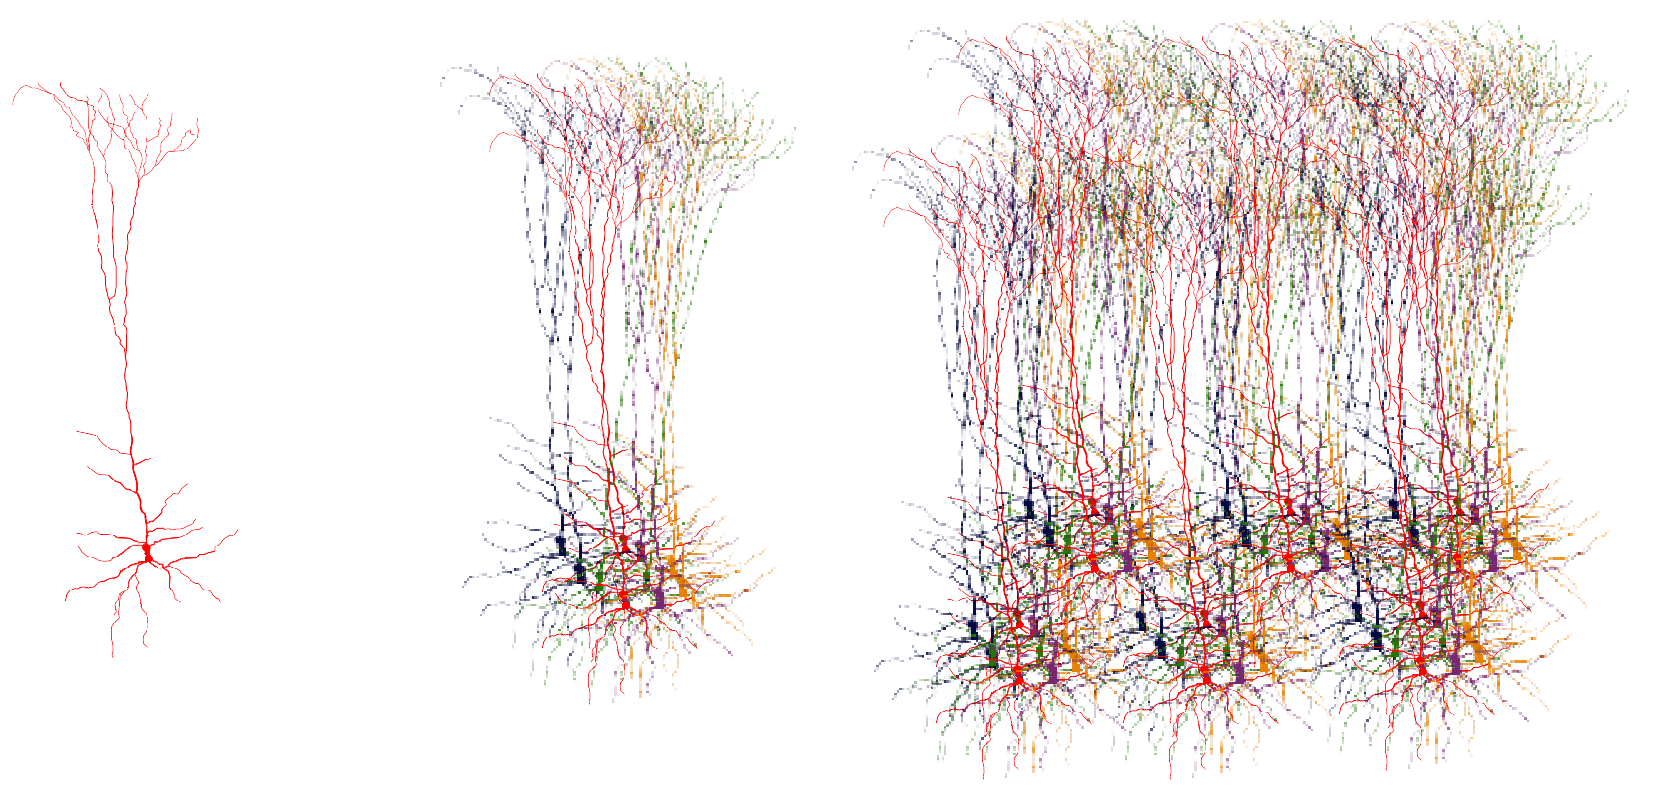
\includegraphics[width=1.0\textwidth]{Biological.png}
    \caption{Organización del tejido cortical. Izquierda: Célula piramidal. La neurona excitatoria más comunmente hallada en el tejido cortical.
    Centro: mini-columna cortical. Un cluster de células neuronales que responden a estímulos de características similares.
    Derecha: Columna Cortical. Un grupo de mini-columnas corticales con campos receptivos de ubicación común.
    Adaptado de (Fabuio, Own work, CC BY 4.0, \url{https://commons.wikimedia.org/w/index.php?curid=60707501)}}
    %\caption{Cortical tissue organization. Left: Pyramidal cell. The most common excitatory neuron in cortical tissue.
    %Center: Cortical mini-column. A cluster on neural cells which responds to stimuli of similar characteristics.
    %Right: Cortical Column. A group of mini-columns with a common receptive field location.
    %Adapted from (Fabuio, Own work, CC BY 4.0, \url{https://commons.wikimedia.org/w/index.php?curid=60707501)}}
    \label{fig:Biological}
\end{figure}

Los márgenes en el diámetro de las columnas corticales se hallan entre 300 y 600 $\mu m$; aún entre diferentes especies cuyos volúmenes cerebrales difieren en un factor de $10^3$. La expansión evolutiva de la corteza cerebral es obtenida con el incremento del área de la superficie cortical por medio de un incremento en el número de columnas corticales y no por un incremento en el tamaño de las columnas individuales \cite{rakic_1995}. Estos hechos sugieren que el tejido cortical está organizado a través de una estructura modular y uniforme. En esta línea de pensamiento, Mouncastle sugirió en 1978 la posibilidad de la existencia de un algoritmo cortical único replicado a través de toda la corteza \cite{mountcastle_1978}.

%Margins in column diameter are between 300 and 600 $\mu m$; even among different species whose brains differ in volume by a factor of $10^3$. The evolutionary cortical brain expansion is achieved due to the expansion in cortical surface area by an increase in the number of cortical columns instead of by an increase in individual column size \cite{rakic_1995}. These facts suggest that cortical tissue is organized in a modular and uniform structure. In accordance, Mountcastle suggested in 1978 that there could be a unique cortical algorithm replicated throughout the neocortex \cite{mountcastle_1978}.

En referencia a la uniformidad de la corteza, Linden y Schreiner listaron una serie de analogías--mayormente neurofisiológicas--entre diferentes cortezas sensoriales, tratando de mostrar que si bien los circuitos corticales auditivos presentan algunas características únicas, sus similitudes con otras regiones sensoriales--como las cortezas visual y la somatosensorial--parecen ser mucho más categóricas \cite{linden_2003}. Primero, a nivel sensorial, el mapeo unidimensional de frecuencia de la cóclea podrían ser análogos a los mapeos bidimensionales que se encuentran en la retina y en la superficie del cuerpo. Segundo, los mapas tonotópicos hallados en el sistema auditivo podrían ser análogos a las organizaciones retinotópicas y somatotópicas halladas en las cortezas visual y somatosensorial respectivamente. Tercero, la configuración de las curvas de respuesta en frecuencia en el sistema auditivo podrían corresponder a la inhibición encontrada en los alrededores de un punto espacial fijando límites en los campos receptivos de las cortezas visual y somatosensorial. También se podría trazar una correspondencia entre la tasa de modulación de amplitud en el sistema auditivo y la sensibilidad al parpadeo de luz en el sistema visual, o la sensibilidad a la vibración de bigotes en el sistema somatosensorial. Finalmente, los campos receptivos auditivos ajustados para el barrido de frecuencia podrían ser análogos a la sensibilidad al movimiento hallada en las cortezas visual y somatosensorial. 

%Linden and Schreiner proposed that although auditory cortical circuits have some unique characteristics, their similarities with other sensory regions--such as visual or somatosensory cortex--seem to be much more categorical \cite{linden_2003}. They proposed a series of analogies: first, at the sensory level, the cochlear one-dimensional frequency map could be analogue to the two-dimensional spatial maps which are found in the retina or body surface. Second, the tonotopic maps found in the auditory system could be analogue to the retinotopic and somatotopic organization found in visual and somatosensory cortices, respectively. Frequency tuning curves in the auditory system could correspond to an inhibition of the spatial surrounding boundaries in visual and somatosensory receptive fields. A correspondence could be drawn between the amplitude modulation rate in the auditory system and the flicker sensitivity in the visual system, or the whisker vibration sensitivity in the somatosensory system. Finally, auditory receptive fields tuned for frequency-sweep, could be analogous to visual and somatosensory motion sensitivity.

Siguiendo en esta línea, \gls{a1} comparte características estructurales comunes con otras cortezas sensoriales \cite{huang_2000, winer_1992, rockel_1980, mitani_1985, mitani_1985A}. Como evidencia nueurofisiológica en favor de la uniformidad de la corteza--aún en la corteza auditiva--podemos decir que circuitos tálamo-corticales recableados para recibir señales visuales en la corteza auditiva de hurones vivos muestran que dicha estructura puede soportar transformaciones tálamo-corticales como intracolumnares vistas en otras modalidades. Cuando las entradas retinales son ruteadas a través del tálamo auditivo, las células corticales auditivas desarrollan propiedades de respuesta visual como selectividad direccional, preferencia en orientación y campos receptivos simples y complejos \cite{sur_1988, angelucci_1998, roe_1992}. Los mapas retinotópicos en términos de afinidad a la orientación con conectividad lateral entre dominios de orientación, emergen en capas superficiales de la corteza auditiva recableada \cite{roe_1990, sur_2000}. Todos estos datos sugieren fuertemente la existencia de un circuito neuronal con capacidades de procesamiento similar para diferentes modalidades. 

%\gls{a1} shares common structural characteristics with other sensory cortices \cite{huang_2000, winer_1992, rockel_1980, mitani_1985, mitani_1985A}. Thalamo-cortical circuits, rewired to receive visual signals in live ferret auditory cortex, show how this structure can support thalamo-cortical and intracolumnar transformations seen in other modalities. When retinal inputs are routed into the auditory thalamus, auditory cortical cells develop visual response properties such as direction selectivity, orientation preference and complex and simple receptive fields \cite{sur_1988, angelucci_1998, roe_1992}. Retinotopic maps, in terms of orientation tuning with lateral connectivity between orientation domains, emerge in superficial layers of the rewired auditory cortex \cite{roe_1990, sur_2000}. These data suggest the existence of neuronal circuitry with similar processing capabilities for different modalities.





\subsection{Fenómenos de Adaptación y Representaciones Dispersas y Distribuidas}

Una de las propiedades funcionales halladas en muchas redes en la corteza es la adaptación a estímulos contextuales \cite{KRAUSE201436,doi:10.1167/16.13.1}. Estos mecanismos mejoran la eficiencia en la codificación de la información sensorial. Por ejemplo, una reducción en las respuestas a sonidos frecuentes por medio de redes inhibitorias puede mejorar la sensibilidad cortical frente a sonidos raros que podrían representar eventos inesperados \cite{Natan2015ComplementaryCO,nachum_2003,Javitt11962}.

%One of the functional properties found in many of these networks is adaptation to contextual stimuli \cite{KRAUSE201436,doi:10.1167/16.13.1}. This mechanism is thought to enhance efficiency in the codification of sensory information. For instance, a reduction in the responses to frequent sounds by means of inhibitory networks, may enhance cortical sensitivity to rare sounds that may represent unexpected events~\cite{Natan2015ComplementaryCO,nachum_2003,Javitt11962}.

Hallazgos recientes en neurociencia muestran que la corteza de mamíferos procesan información por medio de \glspl{sdr}~\cite{barth_2012}. Este mecanismo permite discriminación robusta y con tasas de error bajas en las representaciones de los estímulos minimizando la activación neuronal durante la tarea en relación a los recursos neuronales disponibles para la representación \cite{ahmad_2016}. Hawkins et al. \cite{hawkins_2016} sostienen la hipótesis que uno de los mecanismos que podrían estar involucrados en redes corticales para obtener \glspl{sdr} implica una depolarización parcial y extendida del soma como resultado de activaciones de ramas dendríticas independientes por medio de receptores \gls{nmda} producidas por la excitación de cierto número de sinapsis distantes \cite{antic_2010, major_2013}. Aquellas neuronas parcialmente depolarizadas presentan mayor sensibilidad a estímulos aferentes propiciando inhibición lateral--dentro de una \gls{cc}--y de esta manera evidenciando un fenómeno de adaptación neuronal que devuelve \glspl{sdr} ante secuencias fonéticas conocidas o \glspl{mfe} ante fallas de predicción.

%Finally, recent findings in neuroscience show that mammalian cortex processes information by means of \glspl{sdr}~\cite{barth_2012}. This mechanism allows robust and low-error-rate discrimination of stimuli representations minimizing the neuronal activation during the task in relation to the neural resources available for the representation~\cite{ahmad_2016}. Hawkins et al. \cite{hawkins_2016} hypothetize that one of the mechanisms that might be involved in cortical networks in order to achieve \glspl{sdr} implies the extended depolarization of the soma as the result of independent dendritic \gls{nmda} branch activations produced by the excitation of certain number of distal synapses~\cite{antic_2010, major_2013}.

En este trabajo, las características neurofisiológicas y anatómicas--arriba enumeradas--presentes en la corteza de mamíferos son agrupadas como potencialmente relevantes para sostener el fenómeno de invarianza fonética en la corteza auditiva de mamíferos. Testeamos dichos principios utilizando un modelo computacional biológicamente inspirado y completamente no-supervisado que devuelve una precisión en clasificación fonética similar a la obtenida por las mejores implementaciones de aprendizaje profundo. Por lo tanto, en este trabajo proponemos una ruta alternativa para el manejo de la discriminación fonética basada en la observación de las propiedades funcionales y estructurales de la corteza de mamíferos. 

%In the present work the above mentioned anatomical and neurophysiological features of the mammalian cortex are gathered as potentially relevant in order to attain phonetic invariance in the mammalian auditory cortex. We test those principles using a completely unsupervised and biologically inspired computational model which returns phonetic classification accuracy levels similar to those of state-of-the-art deep pattern classification approaches. We therefore propose an alternative path towards addressing phonetic discrimination based on observing structural and functional properties present in the mammalian cortex.




\section{Implementación}

\subsection{Flujo de Datos}

Nuestro \glsfirst{cstm} simula un parche de tejido cortical en el cerebro de mamíferos. 

La Fig. \ref{fig:DataFlow} muestra el flujo de datos de la información que converge al \gls{el}. Las ondas de sonido son procesadas por el \gls{mrstsa}. Chi T. et al. \cite{chi_2005} desarrollaron un modelo computacional de análisis auditivo inspirado en hallazgos neurofisiológicos y psicoacústicos en etapas tempranas del sistema auditivo. En este trabajo seguimos los lineamientos principales en la implementación de la sección cortical de tal modelo.

%Fig. \ref{fig:DataFlow} shows the data flow of the information converging to the \gls{el}. Sound waves are processed by the \gls{mrstsa}. As mentioned above, Chi T. et al. \cite{chi_2005} developed a computational model of auditory analysis inspired by psychoacoustical and neurophysiological findings in early and central stages of the auditory system. We followed the main guidelines in the implementation of the cortical section of such model.

El algoritmo original tiene una etapa cortical y una subcortical. Para la etapa subcortical, primero un transformada wavelet afín de la señal acústica representa el análisis espectral realizado por el banco de filtros coclear. Segundo, las salidas de los filtros cocleares son transducidos en patrones del nervio auditivo por una etapa de células pilosas consistente en un filtro pasa-altos, una compresión no linear y una membrana de filtro pasa-bajos de fuga. Tercero, una derivada de primer orden con respecto al eje tonotópico seguido por un rectificador de media onda simula la acción de una red de inhibición lateral que se postula como existente en el núcleo coclear, la cual mejora sustancialmente la selectividad en frecuencia del banco de filtros coclear. La salida final de esta etapa se obtiene por medio de la integraciaón sobre una ventana corta, con una constante de 8 ms, simulando la pérdida de fase subsecuente observada en el mesencéfalo.

%The original algorithm has a subcortical and a cortical stage. For the subcortical stage, first an affine wavelet transform of the acoustic signal represents the spectral analysis performed by the cochlear filter bank. Second, the cochlear filter outputs are transduced into auditory-nerve patterns by a hair cell stage consisting of a high-pass filter, a nonlinear compression and a membrane leakage low-pass filter. Third, a first-order derivative with respect to the tonotopic axis followed by a half-wave rectifier simulates the action of a lateral inhibitory network postulated to exist in the cochlear nucleus, which effectively enhances the frequency selectivity of the cochlear filter bank. The final output of this stage is obtained by integrating over a short window, with time constant of 8 ms, mimicking the further loss of phase locking observed in the midbrain.

La etapa cortical simula aspectos de las respuestas de etapas auditivas centrales más altas, especialmente \gls{a1}. Funcionalmente, esta etapa estima el contenido de la modulación espectral y temporal del espectrograma auditivo. Esta etapa, realiza dicha tarea de manera computacional a través de un banco de filtros que son selectivos a diferentes parámetros de modulación espectro temporal que van desde tasas temporales lentas a rápidas y desde escales espectrales estrechas a anchas. Los \glspl{strf} de estos filtros se centran también a diferentes frecuencias a lo largo del eje tonotópico.

%The cortical stage mimics aspects of the responses of higher central auditory stages, especially \gls{a1}. Functionally, this stage estimates the spectral and temporal modulation content of the auditory spectrogram. It does so computationally via a bank of filters that are selective to different spectrotemporal modulation parameters that range from slow to fast rates temporally, and from narrow to broad scales spectrally. The \glspl{strf} of these filters are also centered at different frequencies along the tonotopic axis.

Debido a que en este trabajo incitamos una incorporación parsimoniosa de propiedades neurofisiológicas--principalmente centradas en características de la corteza--decidimos seguir los lineamientos principales de la implementación de la sección cortical en tal modelo.

%In the present work, since we prompt a parsimonious incorporation of neurophysiological properties--mainly centered in cortical features--we followed the main guidelines in the implementation of the cortical section of such model.

\begin{figure}[h!]
    \centering
    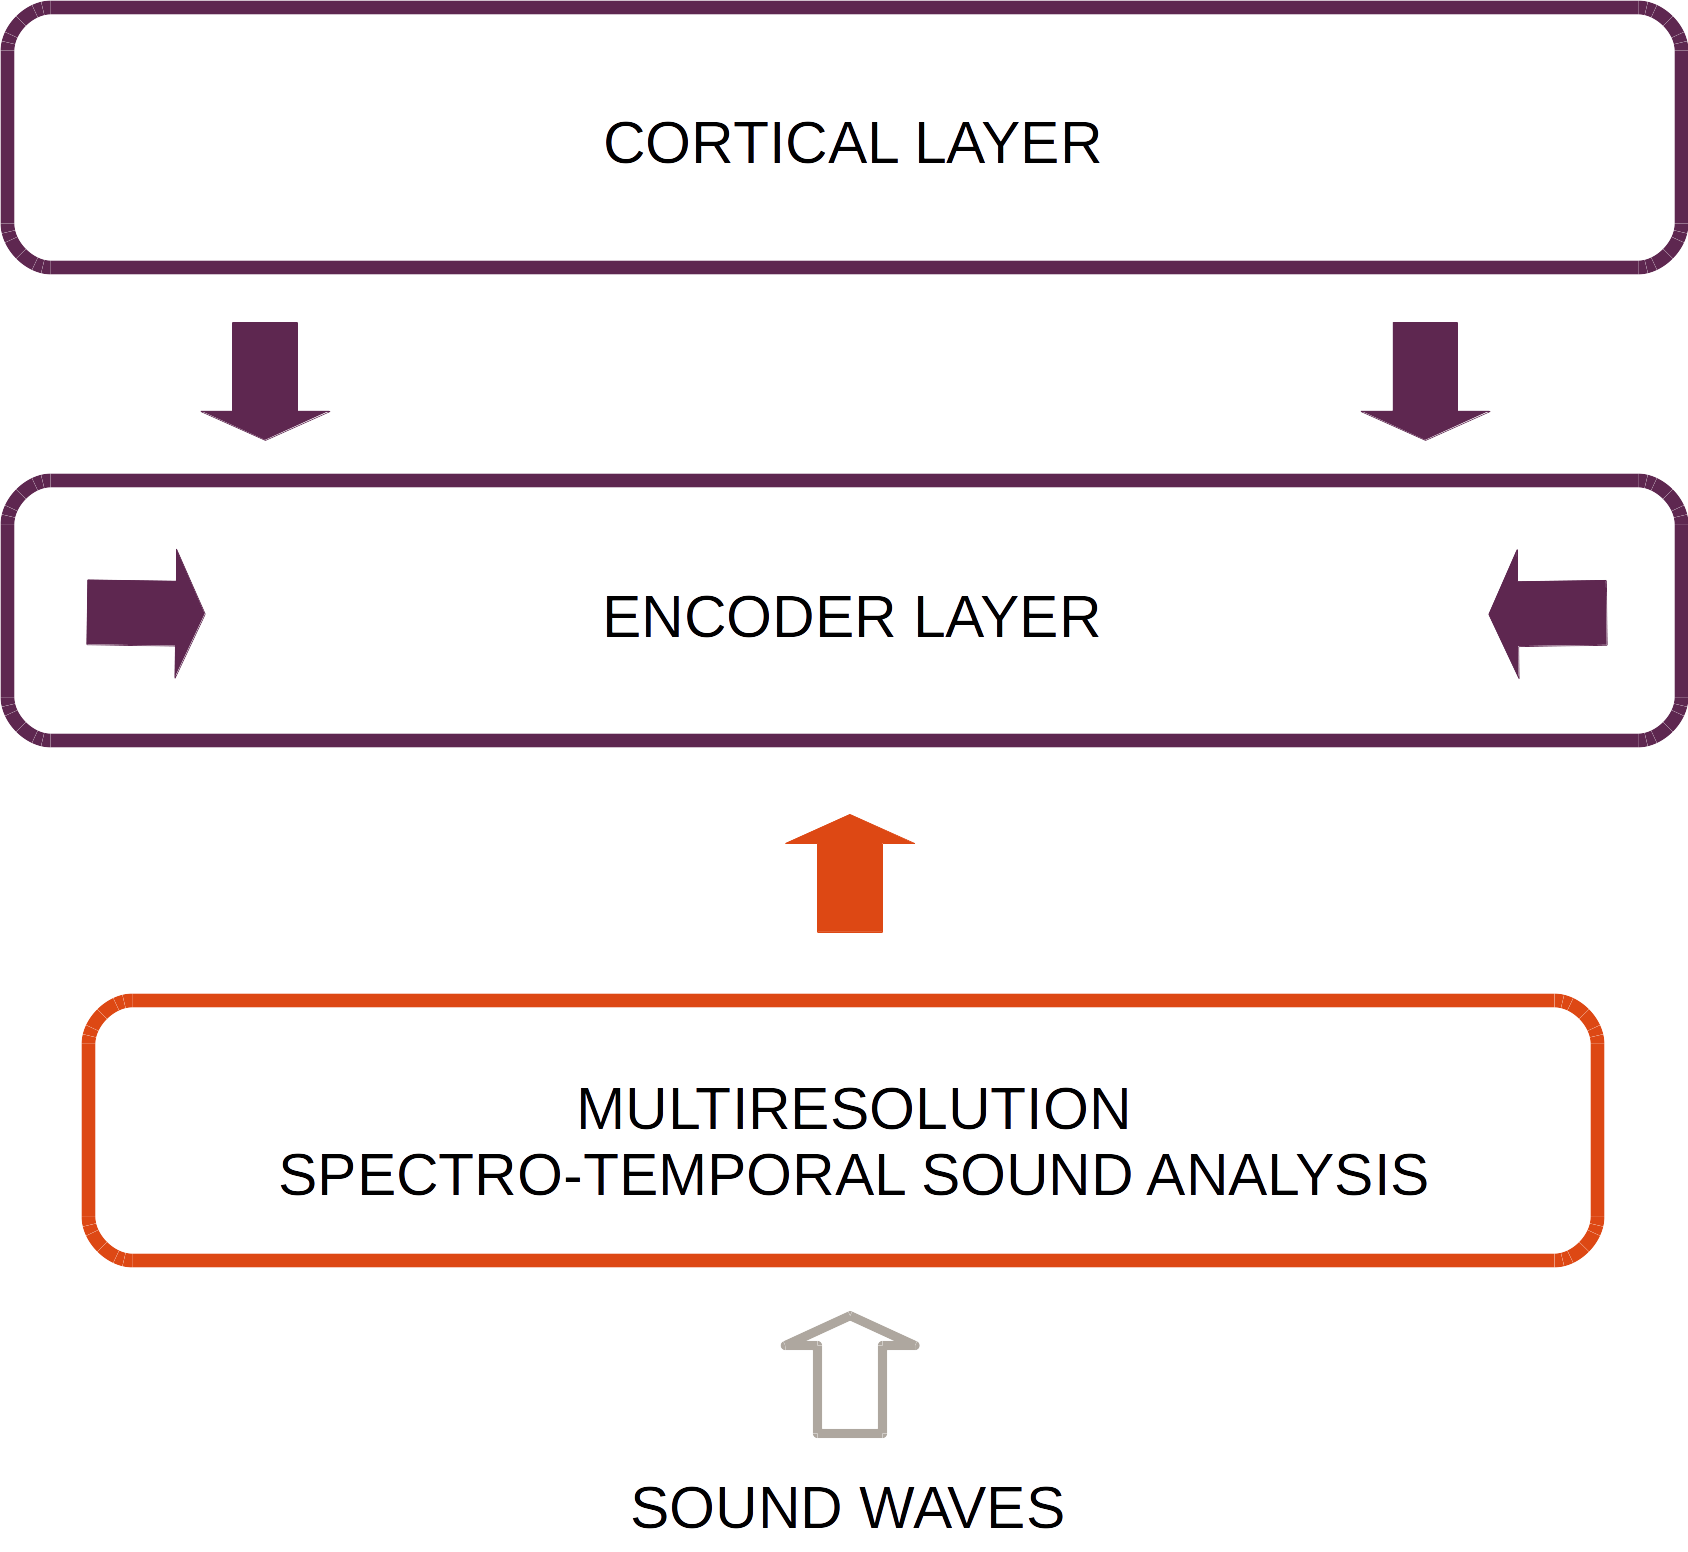
\includegraphics[width=0.5\textwidth]{DataFlow.png}
    \caption{El algoritmo \gls{mrstsa} procesa las ondas de sonido en una secuencia de ventanas temporales y obtiene una secuencia de arreglos de números reales. Tal secuencia de arreglos es recibida por el \gls{el} a través de conexiones aferentes próximas. El \gls{el} también recibe conexiones laterales distantes que traen información de su mismo procesamiento y conexiones apicales distantes que traen información desde otras capas corticales que están por encima del \gls{el}.}
    %\caption{The \gls{mrstsa} processes the sound waves in a sequence of temporal windows and obtains a sequence of arrays of real numbers. Such sequence of arrays is received by the \gls{el} by means of proximal afferent connections. The \gls{el} also receives distal lateral connections which bring information from its self processing and distal apical connections which bring information from other cortical layers above the \gls{el}.}
    \label{fig:DataFlow}
\end{figure}

En cuanto al \gls{el}, simulamos neuronas piramidales con conexiones próximas desde ramificaciones dendríticas aferentes y conexiones distantes desde ramificaciones dendríticas apicales y laterales (Fig. \ref{fig:Pyramidal_Cell}).

%Our \gls{cstm} simulates a patch of cortical tissue in the mammalian brain. We simulate pyramidal cells with proximal connections from afferent dendritic branches and distal connections from lateral and apical dendritic branches (Fig. \ref{fig:Pyramidal_Cell}).

\begin{figure}[h!]
    \centering
    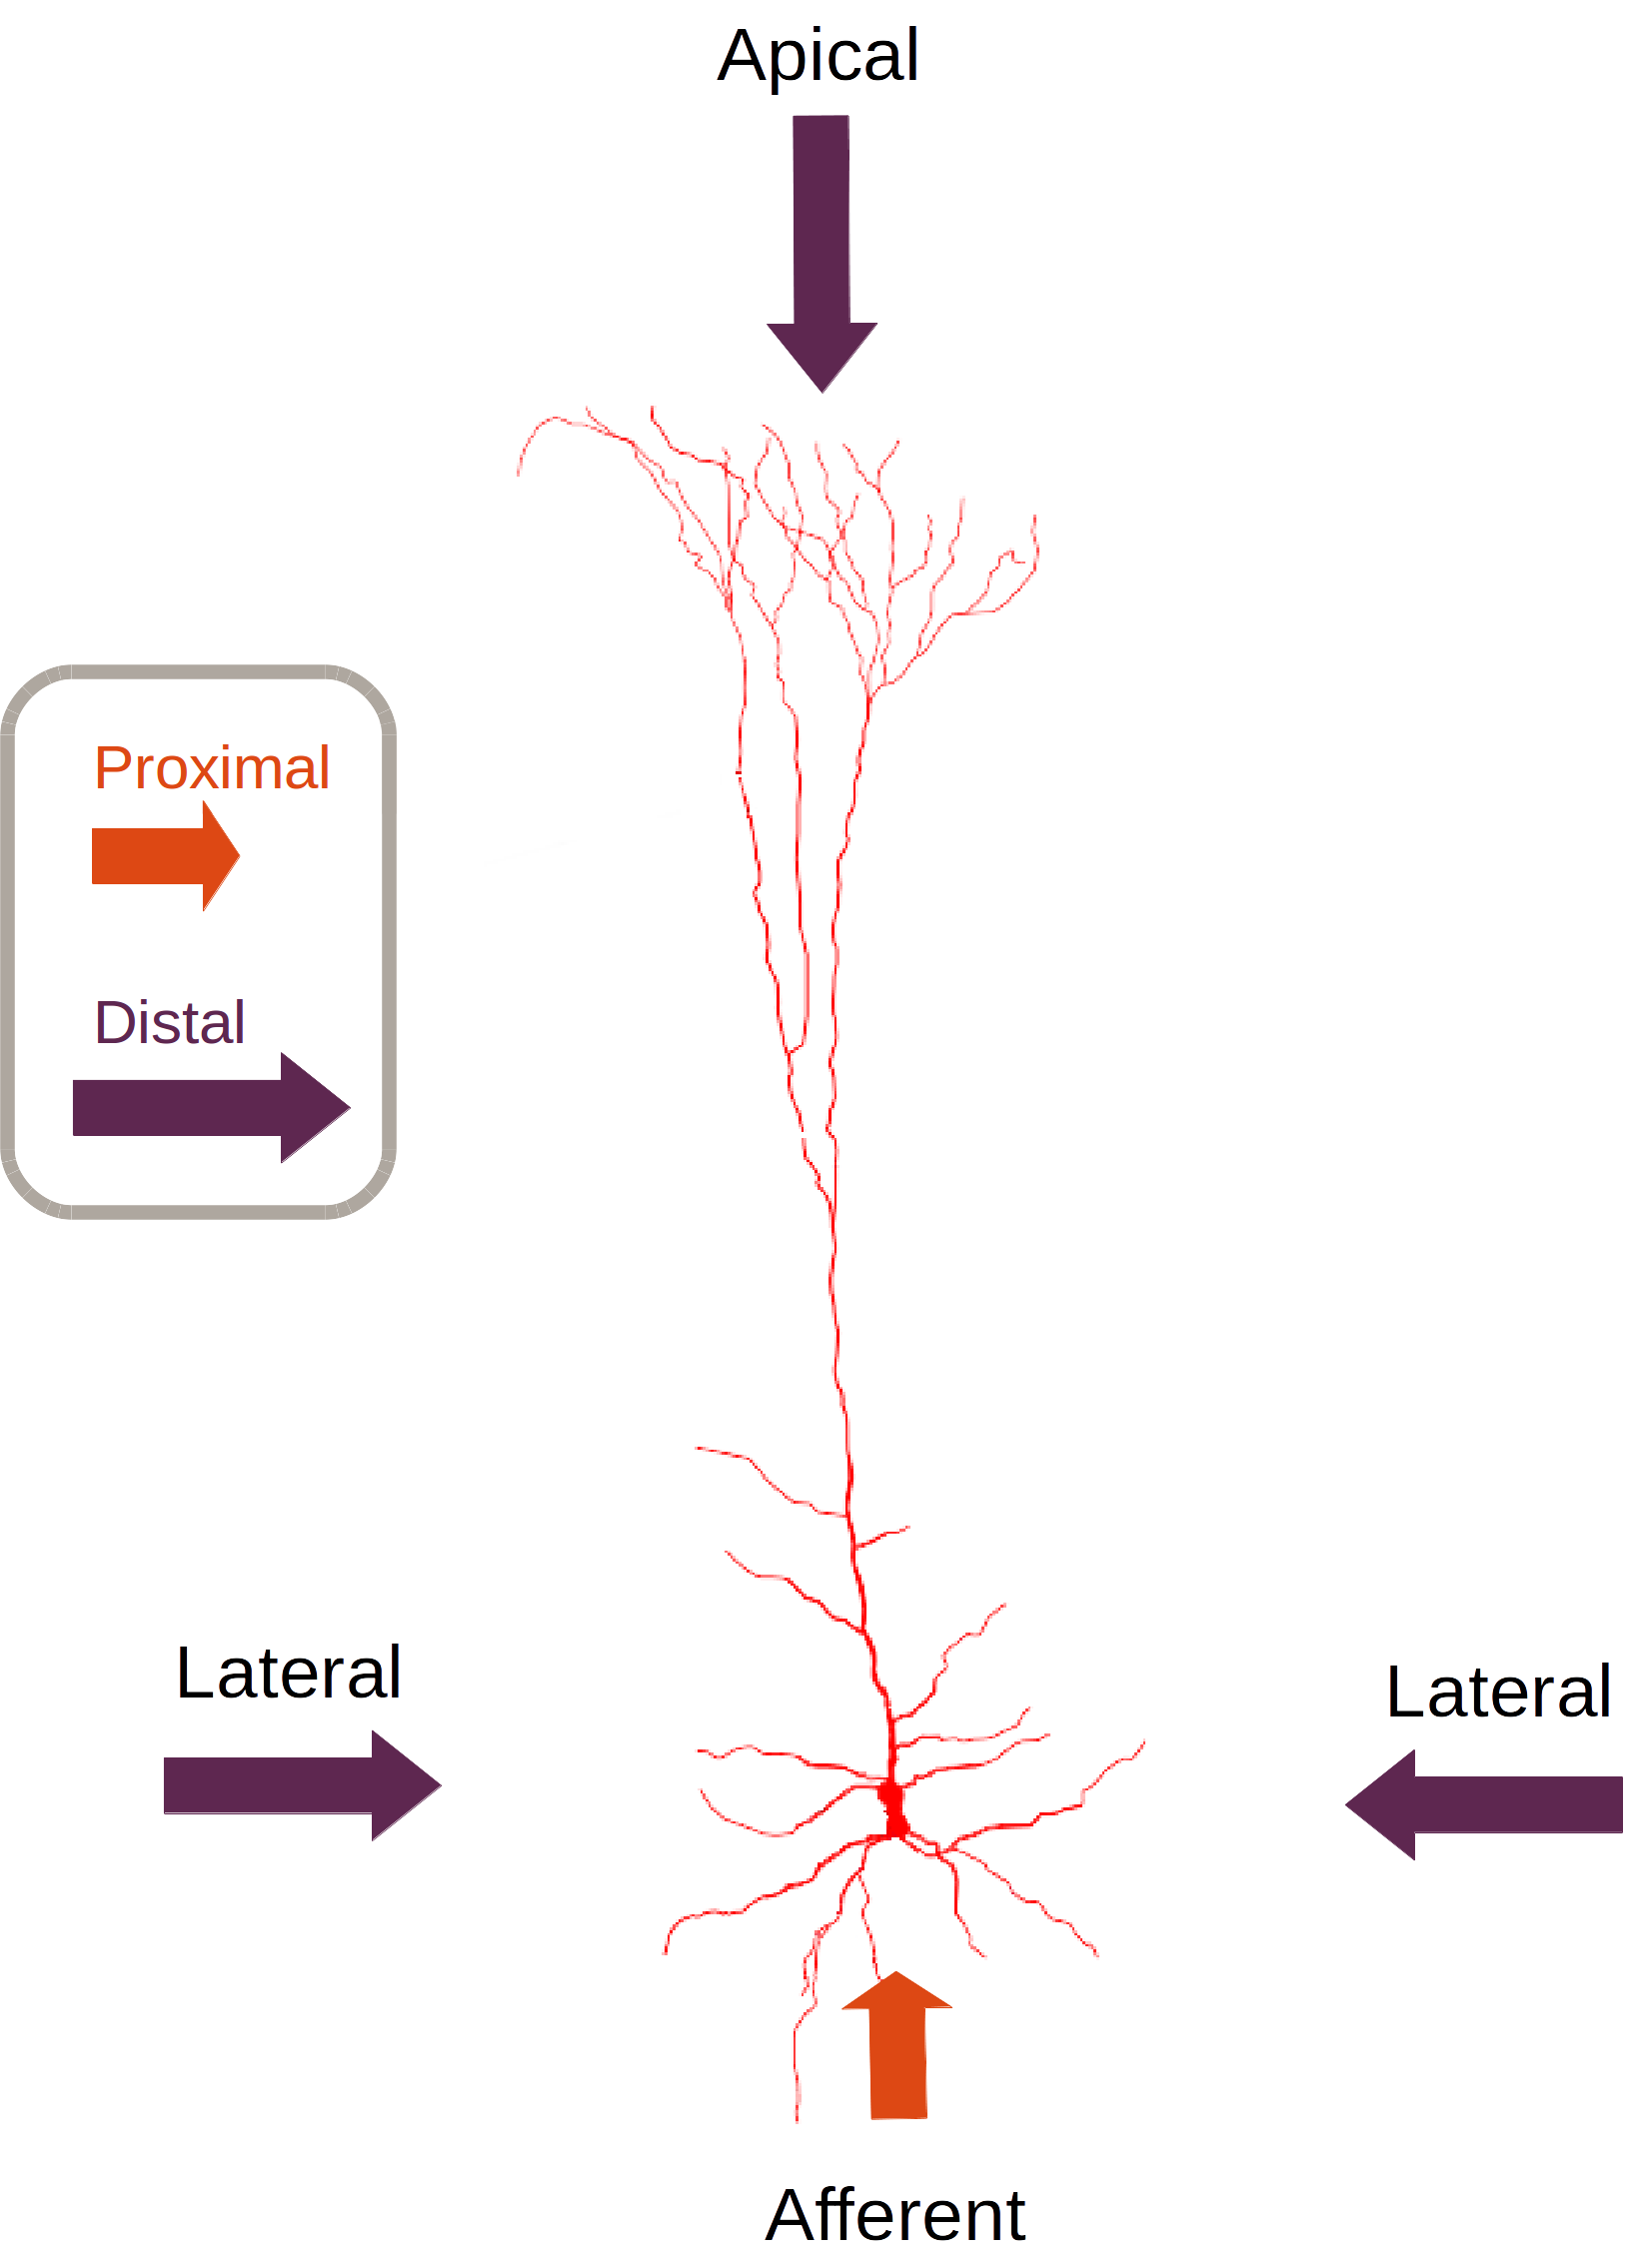
\includegraphics[width=0.4\textwidth]{Pyramidal_Cell.png}
    \caption{Perfil de conectividad de una neurona piramidal en la \gls{el}.
    Las conexiones próximas están compuestas sólo por conexiones aferentes desde el \gls{mrstsa}
    mientras que las conexiones distantes están compuestas por conexiones laterales y apicales desde columnas vecinas y
    desde columnas en otra capa cortical arriba respectivamente.
    Adaptado de (Fabuio - Own work, CC BY 4.0, \url{https://commons.wikimedia.org/w/index.php?curid=60707501)}}
    %\caption{Connectivity profile of a pyramidal neural unit in the \gls{el}.
    %Proximal connections are composed only by afferent connections from the \gls{mrstsa}
    %while distal connections are composed by lateral and apical connections from neighboring columns and
    %from columns in another cortical layer above respectively.
    %Adapted from (Fabuio - Own work, CC BY 4.0, \url{https://commons.wikimedia.org/w/index.php?curid=60707501)}}
    \label{fig:Pyramidal_Cell}
\end{figure}

El \gls{el} es responsable de generar \glspl{sdr} desde las entradas entregadas por la etapa \gls{mrstsa} y desde la historia en la actividad de sus propias \glspl{cc}. El \gls{el} simula un parche de tejido cortical llamado \gls{cl} utilizando una arreglo n-dimensional de estructuras complejas denominadas \glspl{csom} que simulan \glspl{cc} en el cerebro.

%The \gls{el} is responsible for generating \glspl{sdr} from the inputs delivered by the \gls{mrstsa} stage and from the activation history in its own \glspl{cc}. The \gls{el} simulates a patch of cortical tissue called \gls{cl} using an n-dimensional array of complex structures called \glspl{csom} that simulate \glspl{cc} in the brain.

Cada unidad neuronal en una \gls{cc} tiene dos tipos de ramas dendríticas; próximas y distantes. Las ramas dendríticas próximas y distantes conducen a conexiones próximas y distantes en una unidad celular respectivamente. Las conexiones próximas y distantes producen diferentes efectos en la plasticidad y en la activación de una unidad neuronal. Las unidades neuronales en el \gls{el} simulan células piramidales en el tejido cortical en el cerebro. La Fig \ref{fig:Pyramidal_Cell} muestra la conectividad de tales unidades.

%Each cell unit in a \gls{cc} has two types of dendritic branches; proximal and distal. Proximal and distal dendritic branches lead to proximal and distal connections in a cell unit respectively. Proximal and distal connections produce different effects on a neural unit's plasticity and activation. Neural units in the \gls{el} simulates pyramidal cells in cortical tissue in the brain. Fig \ref{fig:Pyramidal_Cell} shows the connectivity profile in such units. 

Cada \gls{cc} en el \gls{el} está conectada con el \gls{mrstsa} que se encuentra debajo de la misma por medio de conexiones aferentes. También se encuentra conectada con \glspl{cc} vecinas--incluida posiblemente ella misma--en el \gls{el} por medio de conexiones laterales y con \glspl{cc} desde otras \glspl{cl} arriba por medio de conexiones apicales. Tal esquema de conexión se muestra en la Fig \ref{fig:DataFlow}.

%Each \gls{cc} in the \gls{el} is connected to the \gls{mrstsa} below by means of afferent connections. It is also connected to neighboring \glspl{cc}--including possibly itself--in the \gls{el} by means of lateral connections and to \glspl{cc} from other \glspl{cl} above by means of apical connections. Such connection scheme is shown in Fig \ref{fig:DataFlow}.

Estímulos aferentes similares activan clusters de neuronas con ubicaciones físicas próximas en una \gls{cc} de la misma manera que información aferente activa mini-columnas en el tejido cortical. Información aferente activa diferentes clusters de unidades en una \gls{cc} estableciendo una primera y grosera aproximación de las características fonéticas abstraídas desde el flujo auditivo de entrada. Nuestro modelo afina tales características groseras por medio de activaciones contextuales previas en la misma \gls{cc} y/o en \glspl{cc} vecinas. Tal información contextual es enviada a cada \gls{cc} por medio de ramas dendríticas laterales que trabajan como elementos de procesamiento independientes en la célula. La activación actual en tales elementos dendríticos afectará la manera en la que las células reciben información aferente futura. Tales conexiones atenúan la actividad de algunas unidades permitiendo sólo activaciones precisas de unidades neuronales específicas en una \gls{cc} aferentemente excitada. Tales activaciones precisas responden al paradigma secuencial aprendido por la red. 

%Similar afferent stimuli activate clusters of neurons with proximal physical locations in a \gls{cc} in the same way that afferent information activates the mini columns found in cortical tissue. Afferent information activates different clusters of units in a \gls{cc} establishing a first and raw approximation of the phonetic features abstracted from the input auditory stream. Our model fine-tunes such raw features by means of previous contextual activations produced in the same and/or in neighboring \glspl{cc}. Such contextual information is sent to each \gls{cc} by means of lateral distal dendritic branches which work as independent processing elements in a cell. Current activation in such dendritic elements will affect the way in which cells receives future afferent information. Such connections damp the activity of some units allowing only the precise activations of specific neural units in an afferently excited \gls{cc}. Such precise activations match the sequential paradigms learned by the network.

Hallazgos recientes en neurociencia \cite{Marques2018} sostienen la idea que la retroalimentación podría potencialmente mejorar las representaciones visuales en tiempo y espacio atenuando la actividad de ciertas células mientras permitiendo la activación de otras que sostienen sus predicciones. En este trabajo sólo implementamos conexiones laterales ya que no existe capa cortical superior de donde traer información apical en la presente implementación. 

%Recent findings in neuroscience \cite{Marques2018} support the idea that feedback could potentially enhance visual representations in time and space damping the activity of certain cells while allowing the activation of others in agreement with its predictions. In this paper we only implement lateral connections since there are no upper layers from which to bring apical information in the present implementation.

Teorías computacionales novedosas han elaborado explicaciones plausibles acerca del rol de las sinapsis distantes relacionadas a los receptores \gls{nmda} \cite{hawkins_2016} combinando esto último con \glspl{sdr} \cite{ahmad_2016}. En nuestro modelo adoptamos un enfoque similar al expuesto en \cite{hawkins_2016} en el cual patrones de activación actuales producen depolarizaciones parciales en ciertas células por medio de conexiones a ramas dendríticas distantes. El estado de depolarización parcial se sostiene en el tiempo para algunas células dentro de los clusters de neuronas que serán excitados aferentemente en el futuro. Las neuronas parcialmente depolarizadas dispararán antes con respecto a otras neuronas en los clusters excitados y así evitarán que esas otras células disparen por medio de inhibición lateral próxima GABAergica, obteniendo así \glspl{sdr}. 

%Novel computational theories have posited a feasible explanation about the role of distal synapses related to \gls{nmda} phenomenon \cite{hawkins_2016} by combining it with \glspl{sdr} \cite{ahmad_2016}. In our model, we adopt a similar approach to the one in \cite{hawkins_2016} in which current activation patterns produce partial depolarization of certain cells by means of distal dendritic branch connections. A state of partial depolarization is sustained in time in some cells within future afferently excited clusters of neurons. Partially depolarized cells fire in advance with respect to other cells in the excited clusters, thereby preventing other cells from firing by means of proximal lateral GABAergic inhibition, obtaining in this way, \glspl{sdr}.

Además, simulamos el crecimiento de sinapsis en ramas dendríticas distantes por medio de mecanismos de \gls{stdp} junto con regulaciones homeostáticas. De esta manera, las sinapsis distantes  serán establecidas sólo entre células piramidales con patrones de activación secuenciales. Los clusters de neuronas excitados aferentemente que no tengan células parcialmente depolarizadas, dispararán masivamente produciendo un \gls{mfe} (ausencia de inhibición) en respuesta a una falla de predicción (estímulo secuencialmente inesperado en el flujo de los datos); de otra manera, dispararán con eventos de disparo normales (inhibición y por lo tanto \glspl{sdr}) cuando el estímulo secuencial es correctamente predicho.

%In addition, we simulate the growth of distal dendritic branch synapses by means of \gls{stdp} mechanisms together with homeostatic regulations. In this way, distal synapses will be established only among pyramidal cells with sequential patterns of activation. Afferently excited clusters which do not have partially depolarized cells, will fire together producing a \gls{mfe} (lack of inhibition) as a response to a prediction fault (unexpected sequential stimuli in the stream of data); otherwise they will respond with normal firing events (inhibition and therefore \glspl{sdr}) when the sequential stimulus is correctly predicted.

Las \glspl{sdr} exhiben propiedades matemáticas interesantes las cuales les dan altos niveles de rechazo al ruido y tolerancia a fallas en neuronas individuales \cite{ahmad_2015}. Estas son características típicas en el tejido cortical donde las células individuales están lejos de ser 100\% confiables y dichas células mueren y se regeneran continuamente. Para simular este fenómeno, incorporamos características estocásticas por medio de las cuales las células neuronales dentro de clusters aferentemente activados son seleccionadas para ser activadas por medio de una distribución probabilística discreta cuyas probabilidades están determinadas por la excitabilidad aferente de las células individuales durante el entrenamiento.

%\glspl{sdr} exhibit interesting mathematical properties which give them high noise rejection and fault tolerance \cite{ahmad_2015}. These are typical characteristics in cortical tissue where individual cells are far from 100\% reliable and the cells die and regenerate continuously. To simulate this phenomenon, we incorporate stochastic characteristics by which neural cells inside afferently activated clusters are chosen to be active by a discrete distribution whose probabilities are determined by the afferent excitability of individual cells during training.

Así, la evolución de la red no predetermina una célula a disparar pero inclina su probabilidad para hacerlo durante el entrenamiento. Adicionalmente y bajo condiciones específicas, las arborizaciónes dendríticas aferentes se auto-activan de manera aleatoria con niveles cuyos valores límites están establecidos por el aprendizaje.

%Hence, the evolution of our network does not predetermine a neuron to fire but biases its probability of doing so during training. Additionally and under specific conditions, afferent dendritic arborizations activate themselves at random with levels whose boundary values are established by learning. 

Se ha mostrado que el overfitting--un fenómeno in el cual un modelo estadístico describe los errores aleatorios o el ruido en vez de la relación que lo subyace--es considerablemente reducido por propiedades estocásticas aplicadas a los procesos de entrenamiento en redes neuronales artificiales (dropout) \cite{JMLR:v15:srivastava14a}.

%It has been shown that overfitting--a phenomenon in which a statistical model describes random error or noise instead of the underlying relationship--is greatly reduced by stochastic properties in training procedures applied to neural networks (dropout)~\cite{JMLR:v15:srivastava14a}.





\subsection{Implementación Algorítmica}

\subsubsection{\glsfirst{mrstsa}}
\label{mrstsa}

Implementamos la etapa inicial del \gls{mrstsa} con la aplicación de la \gls{fft} al vector de audio con una ventana de muestreo diferente para cada resolución. Luego extraemos la densidad espectral de potencia desde cada resolución. Aplicamos \gls{fft} a los archivos de audio con un período de muestreo de 8 milisegundos, para ello utilizamos el paquete FFTW \cite{FFTW05, fftw} con ventanas temporales de 8, 16, 32, 64 y 128 milisegundos. De esta manera obtenemos un análisis espectral de la señal de audio de resolución múltiple con alta resolución espectral y baja resolución temporal para ventanas grandes y vice versa. Tales diferencias en las ventanas temporales en la aplicación de la \gls{fft} incorporan--al mismo tiempo--filtros pasa-bajo de fuga con una constante de tiempo diferente para cada resolución representando la pérdida de fase en el nervio auditivo. Luego aplicamos \gls{mfb} con 128 elementos a cada espectro a los fines de representar el análisis espectral realizado por el banco de filtros cocleares (Fig.\ref{fig:MRSTSA}).

%We implemented the initial stage in the \gls{mrstsa} with the application of \gls{fft} to the audio vector with a different sample window for each resolution. We then extracted the power spectral density from each resolution. We applied \gls{fft} to the audio files with a sample period of 8 milliseconds, to that end we used the FFTW package \cite{FFTW05, fftw} with time windows of 8, 16, 32, 64 and 128 milliseconds. In this way we obtained a multiresolution spectral analysis of the audio signal, with high spectral and low temporal resolution for wider sample windows and vice versa. Such different time windows in the \gls{fft}, incorporated--at the same time--leakage low-pass filters with a time constant for each resolution accounting for decrease of phase-locking in the auditory nerve. We then applied a \gls{mfb} with 128 elements to each spectrum in order to represent the spectral analysis performed by the cochlear filter bank (Fig.\ref{fig:MRSTSA}).

\begin{figure}[h!]
    \centering
    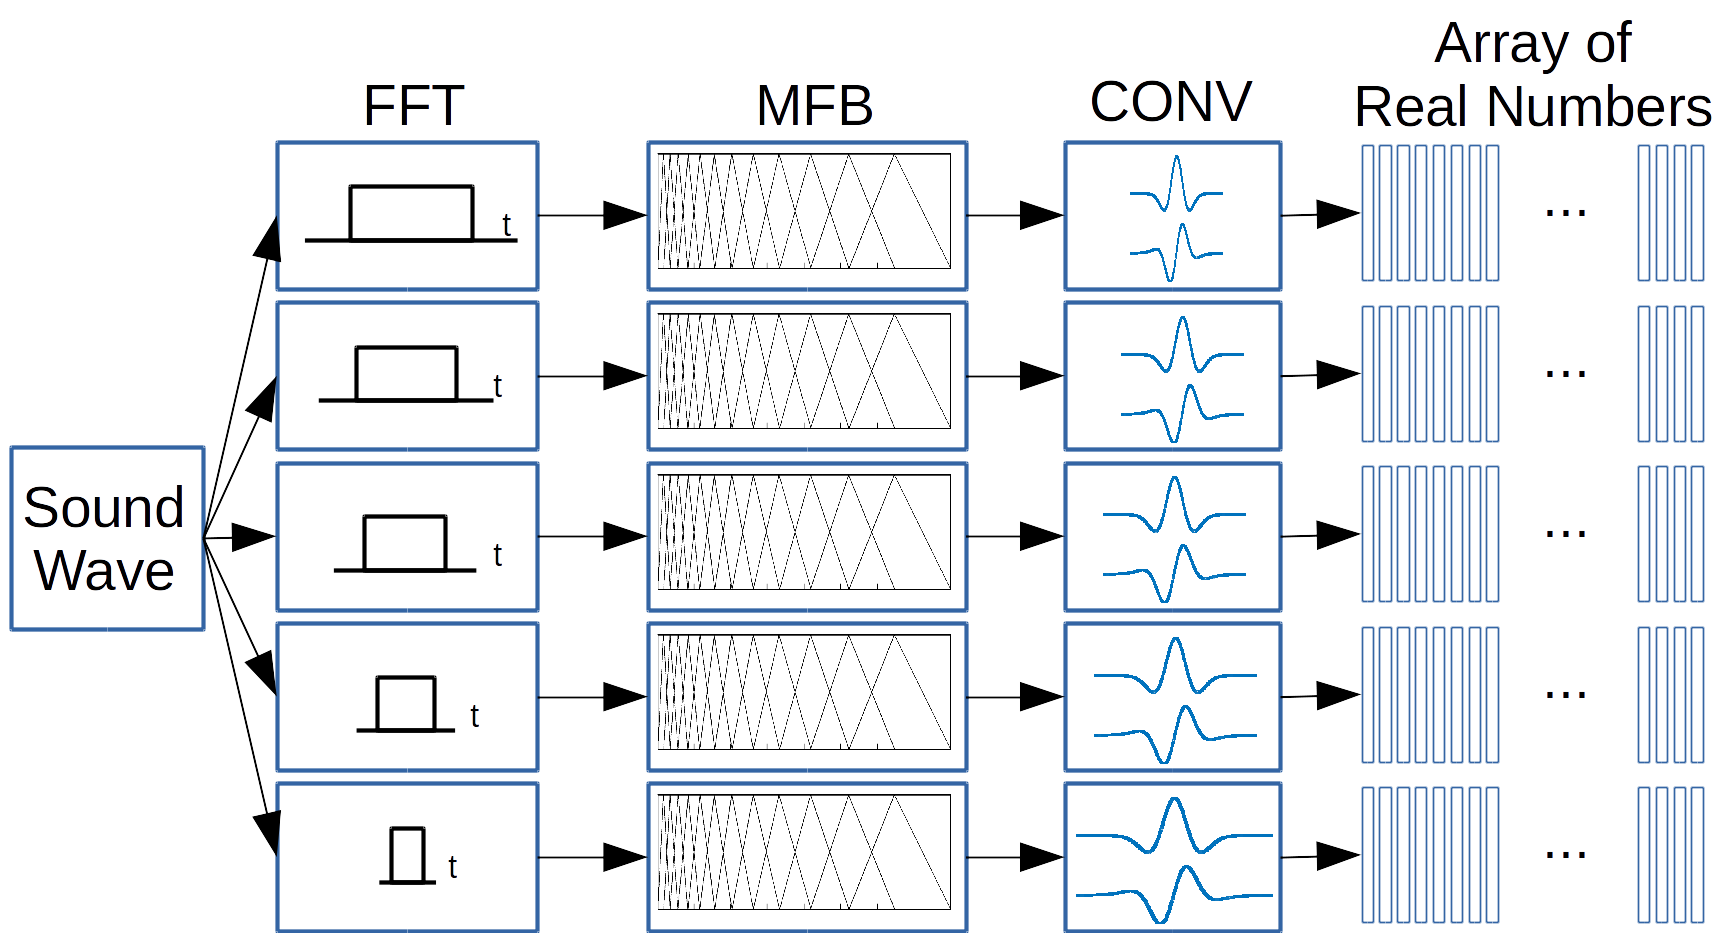
\includegraphics[width=0.8\textwidth]{MRSTSA.png}
    \caption{Algoritmo \glsfirst{mrstsa}. Las ondas de sonido son procesadas por \glspl{fft} con ventanas de tiempo diferentes, luego cada espectro es procesado por
    un \glsfirst{mfb} y cada resolución es convolucionada con una señal compleja con un coeficiente diferente. Luego, el coeficiente de cada filtro
    es obtenido computando el módulo desde la convolución y aplicando control automático de ganancia.}
    %\caption{\glsfirst{mrstsa} algorithm. Sound waves are processed by \glspl{fft} with different time windows, then each spectrum is processed by
    %a \glsfirst{mfb} and each resolution is convolved with a complex signal with a different coefficient. Then, each filter coefficient
    %is obtained computing the modulus from the convolution and then applying a authomatic gain control.}
    \label{fig:MRSTSA}
\end{figure}

Luego, convolucionamos cada resolución obtenida en el último paso a lo largo de su eje tonotópico con una función multiresolución compleja cuya parte real es un sobrero Mexicano simétrico y su parte imaginaria es su transformada antisimétrica de Hilbert. Los coeficientes de la función son 10 para la ventana de tiempo de 8 ms, 8 para la ventana de tiempo de 16 ms, 6 para la ventana de tiempo de 32 ms, 4 para la ventana de tiempo de 64 ms y 2 para la ventana de tiempo de 128 ms (Fig.\ref{fig:MRSTSA}). Con esta estrategia incorporamos el fenómeno de simetría \cite{shamma_1993}, ancho de banda \cite{schreiner_1990} y selectividad a la modulación de frecuencia \cite{shamma_1993,heil_1992,mendelson_1985} hallada en \gls{a1} e incorporado en el algoritmo original \cite{wang_1995}.

%Then, we convolved each resolution obtained in the last step along its tonotopic axis with a complex multiresolution function whose real part was a symmetric Mexican hat function and its imaginary part was its antisymmetric Hilbert transform. The function coefficients are 10 for the 8 ms time window, 8 for the 16 ms time window, 6 for the 32 ms time window, 4 for the 64 ms time window and 2 for the 128 ms time window (Fig.\ref{fig:MRSTSA}). With this strategy we incorporated the phenomena of symmetry \cite{shamma_1993}, bandwidth \cite{schreiner_1990} and frequency modulation selectivity \cite{shamma_1993,heil_1992,mendelson_1985} found in \gls{a1} and incorporated in the original algorithms \cite{wang_1995}.

Obtuvimos la magnitud de cada convolución y aplicamos normalización a cada ventana de tiempo como un control automático de ganancia para priorizar la información entregada por la configuración espectral y no por los valores absolutos entregados por los filtros. Por medio de este mecanismo estamos teniendo en cuenta las propiedades químicas y mecánicas de las células poliosas en el oído interno de los mamíferos las cuales constituyen un mecanismo de transducción el cual parece adaptarse a la historia reciente en los estímulos de manera que puede afectar su ganancia \cite{eatock_2000,holt_2000,le_goff_2005}. Decidimos ser conservativos y no incluir la dimensión de intensidad de sonido sólo incluyendo la silueta en las respuestas de los filtros. 

%We obtained the magnitude of each convolution and applied normalization to each time window as a mean of automatic gain control in order to prioritize the information delivered by the spectral configuration and not the absolute values delivered by the filters. By means of this constraint we account for the mechanical and chemical properties of hair cells in the mammalian inner ear which constitute a transduction mechanism that appears to adapt to recent stimulus history in a way that can affect its gain \cite{eatock_2000,holt_2000,le_goff_2005}. We decided to be conservative, not including sound intensity dimension but just the shape of the filter responses.

Por medio de este procedimiento desde el archivo de audio obtuvimos una respuesta multiresolución espectro-temporal compuesta por un arreglo de 128 columnas--una columna por filtro--y 5 filas--una fila por resolución--con números reales cuyo rango se encuentra entre 0 y 1, para cada paso de tiempo.

%By this procedure we obtained from the audio file a multiresolution spectro-temporal response composed by an array of 128 columns--one column per filter--and 5 rows--one row per resolution--with real numbers which range from 0 to 1, for each time step.




\subsubsection{Plasticidad en las conexiones dendríticas próximas del \glsfirst{el}}
\label{proximal_dendrites}

En referencia a las conexiones próximas en el \gls{el}, cada unidad neuronal en una \gls{cc} tiene el mismo conjunto de conexiones próximas al \gls{mrstsa} (Fig. \ref{fig:DataFlow}). Dicha situación es mostrada en la Fig. \ref{fig:EncoderProximalConnections} y tales conexiones constituyen un espacio multidimensional de números reales (Fig. \ref{fig:MRSTSA}). A los fines de adquirir la distribución estadística en tal espacio real multidimensional utilizamos un \gls{som} multidimensional en cada columna cortical cuyo algoritmo es delineado en Alg. \ref{csom_proximal_synapses}. Cada unidad neuronal tiene un peso sináptico por dimensión de entrada y el conjunto de pesos sinápticos en una unidad neuronal determina su posición en el espacio de entrada. Tales pesos sinápticos tratan de copiar los eventos de los vectores de entrada a medida que suceden en el espacio de entrada.

%In reference to proximal connections in the \gls{el}, each neural unit in a \gls{cc} has the same set of proximal connections to the \gls{mrstsa} (Fig. \ref{fig:DataFlow}). This situation is depicted in Fig. \ref{fig:EncoderProximalConnections} and such connections constitute a multidimensional space of real numbers (Fig. \ref{fig:MRSTSA}). In order to acquire the statistical distribution in such multidimensional real space we use a multidimensional \gls{som} in each cortical column whose algorithm is depicted in Alg. \ref{csom_proximal_synapses}. Each neural unit has a synaptic weight per input dimension and the set of synaptic weights in a neural unit determines its position in the input space. Such synaptic weights try to copy the input vector events as they happen in the input space. 

\begin{figure}[h!]
    \centering
    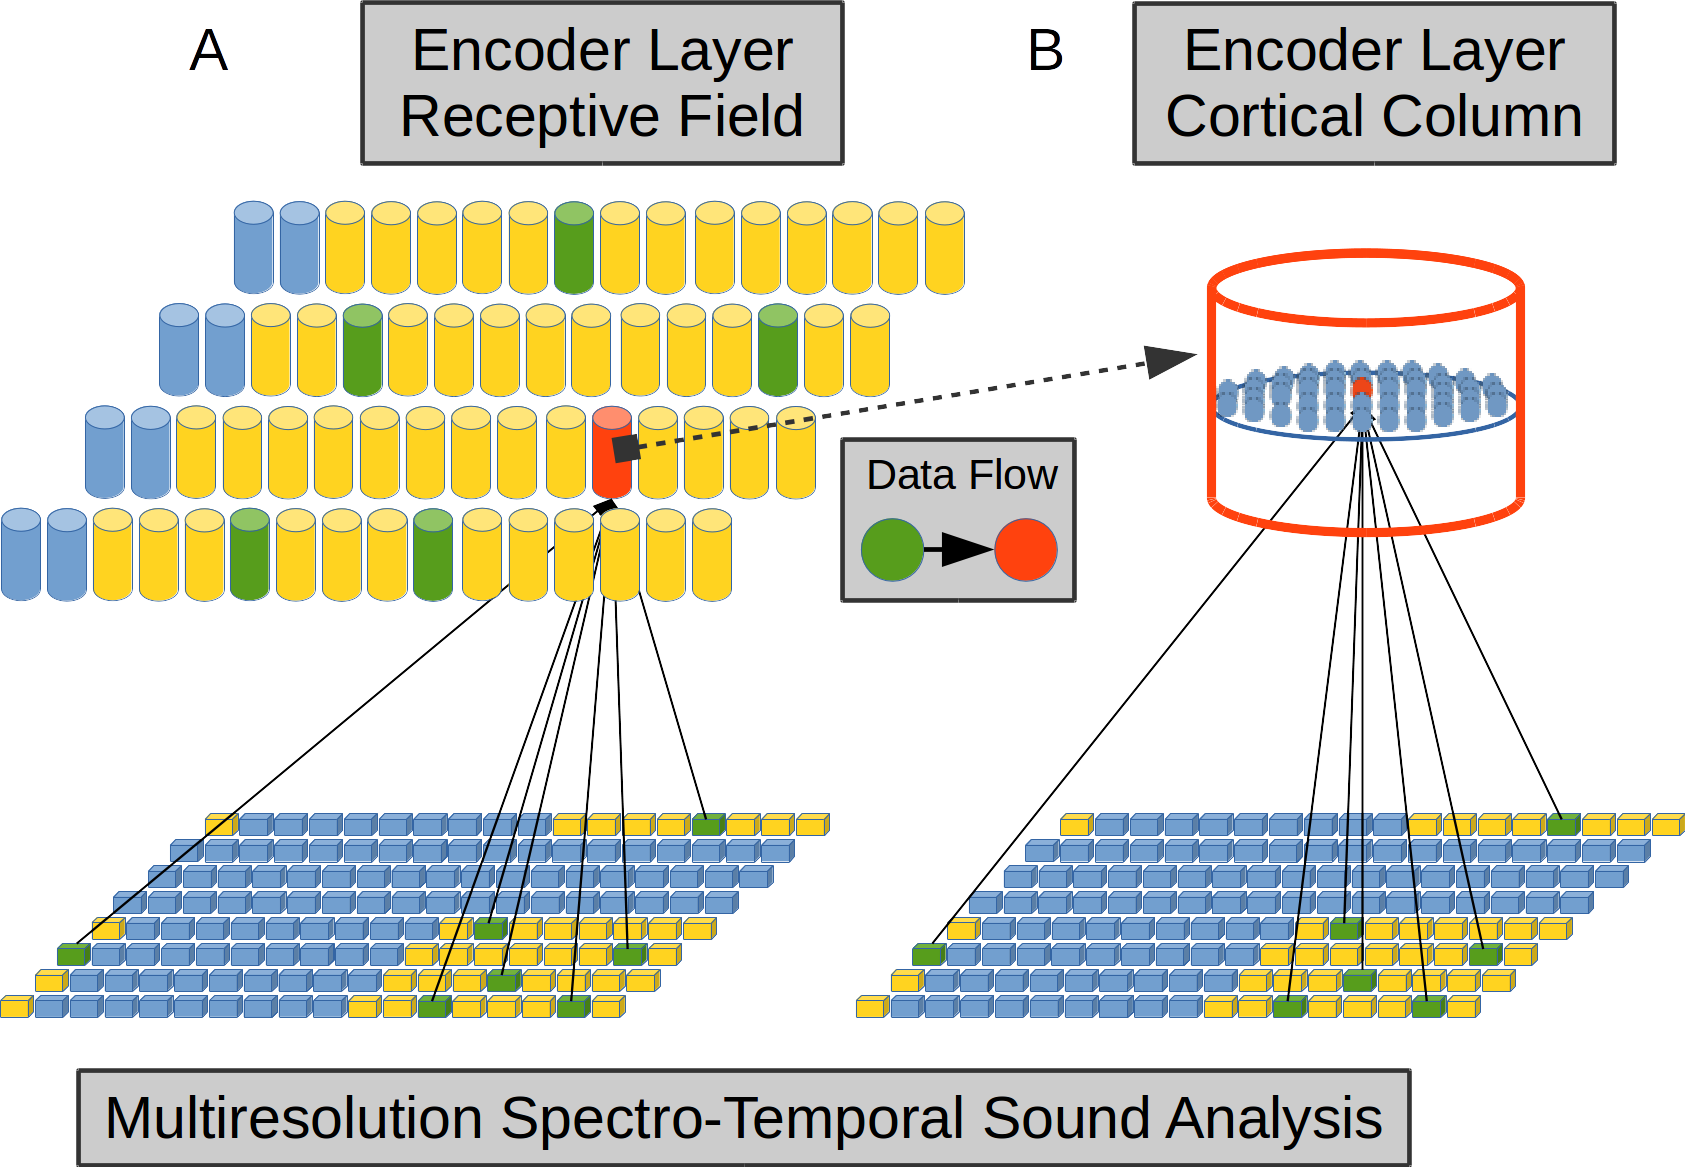
\includegraphics[width=0.6\textwidth]{EncoderProximalConnections.png}
    \caption{Conexiones próximas del \glsfirst{el}. Cada \gls{cc} en el \gls{el}--ejemplificada aquí en rojo--tiene su campo receptivo sobre el \gls{mrstsa}--en amarillo.
    (A) Un conjunto de componentes del \gls{mrstsa}--en verde dentro del campo receptivo--es elegido aleatoriamente para estar conectado con tal \gls{cc}.
    (B) Cada unidad neuronal en tal \gls{cc} está conectada con el mismo conjunto de componentes del \gls{mrstsa}.}
    %\caption{\glsfirst{el} proximal connections. Each \gls{cc} in the \gls{el}--exemplified here in red--has its receptive field over the \gls{mrstsa}--in yellow.
    %(A) A set of \gls{mrstsa} components--in green inside the receptive field--is randomly chosen to be connected with such \gls{cc}.
    %(B) Each neural unit in such \gls{cc} is connected with the same set of \gls{mrstsa} components.}
    \label{fig:EncoderProximalConnections}
\end{figure}

\begin{algorithm}
	\caption{\texttt{Plasticidad en Sinápsis Próximas}. Este algoritmo (un \gls{som}) es un algoritmo de clusterizado no supervisado que distribuye una distribución multidimensional continua en una distribución multidimensional discreta de unidades \cite{Kohonen:1989:SAM:69371, kohonen_2082}. Des esta manera se termina con un arreglo de unidades de $m$ dimensiones en el que cada unidad representa un conjunto de vectores desde una distribución continua en un espacio de entrada de $n$ dimensiones. Generalmente, $m < n$ a los fines de reducir la dimensionalidad en la representación discreta. Incorporamos tal restricción a nuestro algoritmo columnar.}
	%\caption{\texttt{Plasticity in Proximal Synapses}. This algorithm (a \gls{som}) is an unsupervised clustering algorithm which distributes a continuous multidimensional distribution in a discrete multidimensional distribution of units \cite{Kohonen:1989:SAM:69371, kohonen_2082}. In this way we ended up with an array of units of $m$ dimensions in which each unit represents a set of vectors from the continuous distribution in an input space of $n$ dimensions. Generally, $m < n$ in order to reduce the dimensionality in the discrete representation. We added such restriction in our columnar algorithm.}
\label{csom_proximal_synapses}
\begin{algorithmic}[1]
	\STATE{given an \texttt{input} vector, find the nearest \texttt{unit} to such \texttt{input} vector in the input space}
	\STATE{move such \texttt{unit} towards the \texttt{input} vector in the input space (the magnitude of such movement depends on the learning rate)}
	\STATE{also move neighbor \texttt{units} to the nearest one towards the \texttt{input} vector (the magnitude of such movement depends on the learning rate and on a neighborhood measure over the topology of the network of units)}
\end{algorithmic}
\end{algorithm}

La Fig. \ref{fig:SOM} muestra una red bi-dimensional que es un enrejado de 35 por 35 (1225) unidades. La geometría bidimensional de la red tratará de copiar la semántica de la distribución estadística embebida en el espacio de entrada. Es decir, todos los eventos estadísticos en la entrada tendrán una unidad representativa en la red. La estructura bidimensional de la red hará su mejor esfuerzo por encontrar la estructura semántica embebida en el espacio de entrada tridimensional.

%Fig. \ref{fig:SOM} shows a bi-dimensional network which is a lattice of 35 by 35 (1225) units. The bi-dimensional geometry of the network will try to copy the semantic of the statistical distribution embedded in the input space. That is, all the statistical events in the input will have a representative unit in the network. The bi-dimensional structure of the network will do the best in order to find the semantical structure embedded in the three-dimensional input space. 

\begin{figure}[h!]
    \centering
    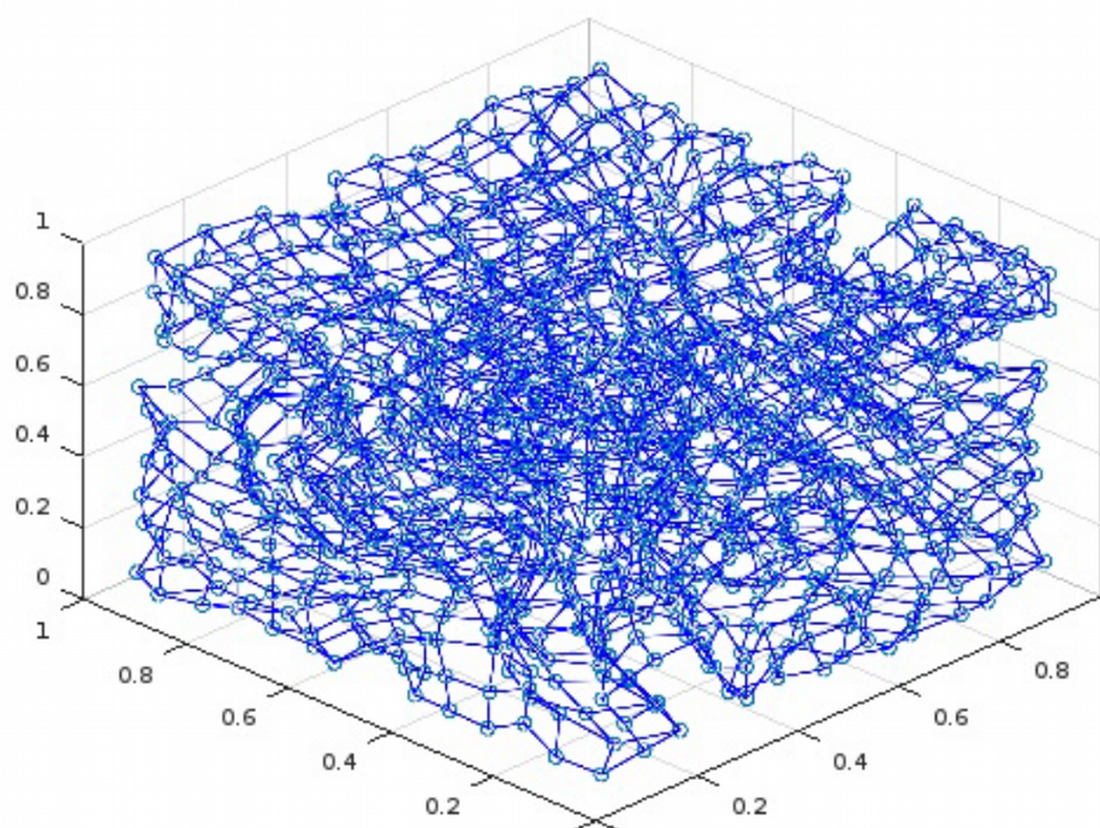
\includegraphics[width=0.4\textwidth]{SOM.png}
    \caption{\glsfirst{som}. En la entrada, los vectores son generados por una distribución cúbica unitaria tridimensional uniforme.
    El arreglo de unidades neuronales es un enrejado bidimensional de 35 por 35 unidades el cual--por medio del Alg. \ref{csom_proximal_synapses}--
    se trata de adaptar a la geometría de entrada para representar los vectores de entrada tan fielmente como sea posible.
    Las unidades neuronales se distribuyen de acuerdo con la distribución estadística en el espacio de entrada.}
    %\caption{\glsfirst{som}. In the input, vectors are generated by a unit cube three-dimensional uniform distribution.
    %The array of neural units is a bi-dimensional lattice of 35 by 35 units which--by means of Alg. \ref{csom_proximal_synapses}--
    %tries to adapt to the input geometry in order to represent the input vectors as faithfully as possible.
    %The neural units are distributed in accordance with the statistical distribution in the input space.}
    \label{fig:SOM}
\end{figure}

Nuestra implementación del \gls{som} se llama \gls{csom}. El algoritmo \gls{csom} refleja interacción intra-columnar lateral próxima, \gls{ltp} y \gls{ltd}. Este algoritmo también disocia las entradas dendríticas próximas de las dendritas distantes, ya que modifica las conexiones próximas siguiendo la distribución estadística desde el \gls{mrstsa} independientemente de las unidades que disparan en tal \gls{cc}. Esta independencia en la plasticidad de las entradas dendríticas próximas es sostenida por la propiedad hallada en el tejido cortical por medio de la cual existe plasticidad dendrítica en el contexto de la depolarización parcial del soma \cite{reiter_1998}--es decir, sin un \gls{ap}.

%We call our implementation of the \gls{som} algorithm, \gls{ssom}. The \gls{ssom} algorithm accounts for proximal lateral intra-column interaction, \gls{ltp} and \gls{ltd}. It also dissociates proximal dendritic inputs from distal dendrites, since it modifies proximal connections following the statistical distribution from the \gls{mrstsa} independently of the units that fire in such \gls{cc}. This independence in the plasticity of the proximal dendritic inputs is supported by the property found in cortical tissue by means of which there is dendritic plasticity in the context of partial depolarization of the soma \cite{reiter_1998}--that is, without an \gls{ap}.

El término \textit{static} viene del hecho de que los patrones aprendidos desde las dendritas aferentes próximas no cuentan para el contexto histórico en la evolución dinámica del algoritmo.

%The term \textit{static} comes from the fact that the patterns learned from proximal afferent dendrites do not account for the contextual history in the dynamic evolution of the algorithm.






\subsubsection{Plasticidad en las conexiones dendríticas distantes del \glsfirst{el}}
\label{distal_dendrites}

En término de las ramas dendríticas distantes, cada \gls{cc}--en este caso ejemplificamos tal \gls{cc} en rojo en la Fig. \ref{fig:DistalDendrites}--en el \gls{el} está conectada con otra \gls{cc}--en verde en la Fig \ref{fig:DistalDendrites}--por medio de tales ramas dentro del campo receptivo de la \gls{cc}--en amarillo en la Fig. \ref{fig:DistalDendrites}--desde el mismo \gls{el} o desde otra \gls{cl} encima del \gls{el}. Cada vínculo entre la \gls{cc} en rojo y una \gls{cc} en verde--Fig. \ref{fig:DistalDendrites} A--simboliza el hecho de que cada unidad celular en la \gls{cc} en rojo se encuentra vinculada con un subconjunto diferente de unidades celulares en la \gls{cc} en verde--Fig. \ref{fig:DistalDendrites} B. Tal sub-conjunto de células--aleatoriamente escogidas--constituye cierto porcentaje del número total de células en la \gls{cc}. Tal porcentaje es un parámetro ajustable para el modelo y determina el número de conexiones potenciales en cada célula en la \gls{cc} en rojo con respecto a una \gls{cc} en verde en la Fig. \ref{fig:DistalDendrites} B.

%In terms of distal dendritic branches, each \gls{cc}--in this case we exemplify such \gls{cc} in red in Fig. \ref{fig:DistalDendrites}--in the \gls{el} is connected to other \glspl{cc}--in green in Fig \ref{fig:DistalDendrites}--by means of such branches inside the \gls{cc} receptive field--in yellow in Fig. \ref{fig:DistalDendrites}--from the same \gls{el} and from another \gls{cl} above. Each link between the red \gls{cc} and a green \gls{cc}--Fig. \ref{fig:DistalDendrites} A--symbolizes the fact that each cell unit in the red \gls{cc} is linked with a different subset of cell units in the green \gls{cc}--Fig. \ref{fig:DistalDendrites} B. Such subset of--random chosen--cells constitutes certain percentage from the total number of cells in the \gls{cc}. Such percentage is a tunable parameter for the model and determines the number of potential connections each cell in the red \gls{cc} has with respect to a green \gls{cc} in Fig. \ref{fig:DistalDendrites} B.

\begin{figure}[h!]
    \centering
    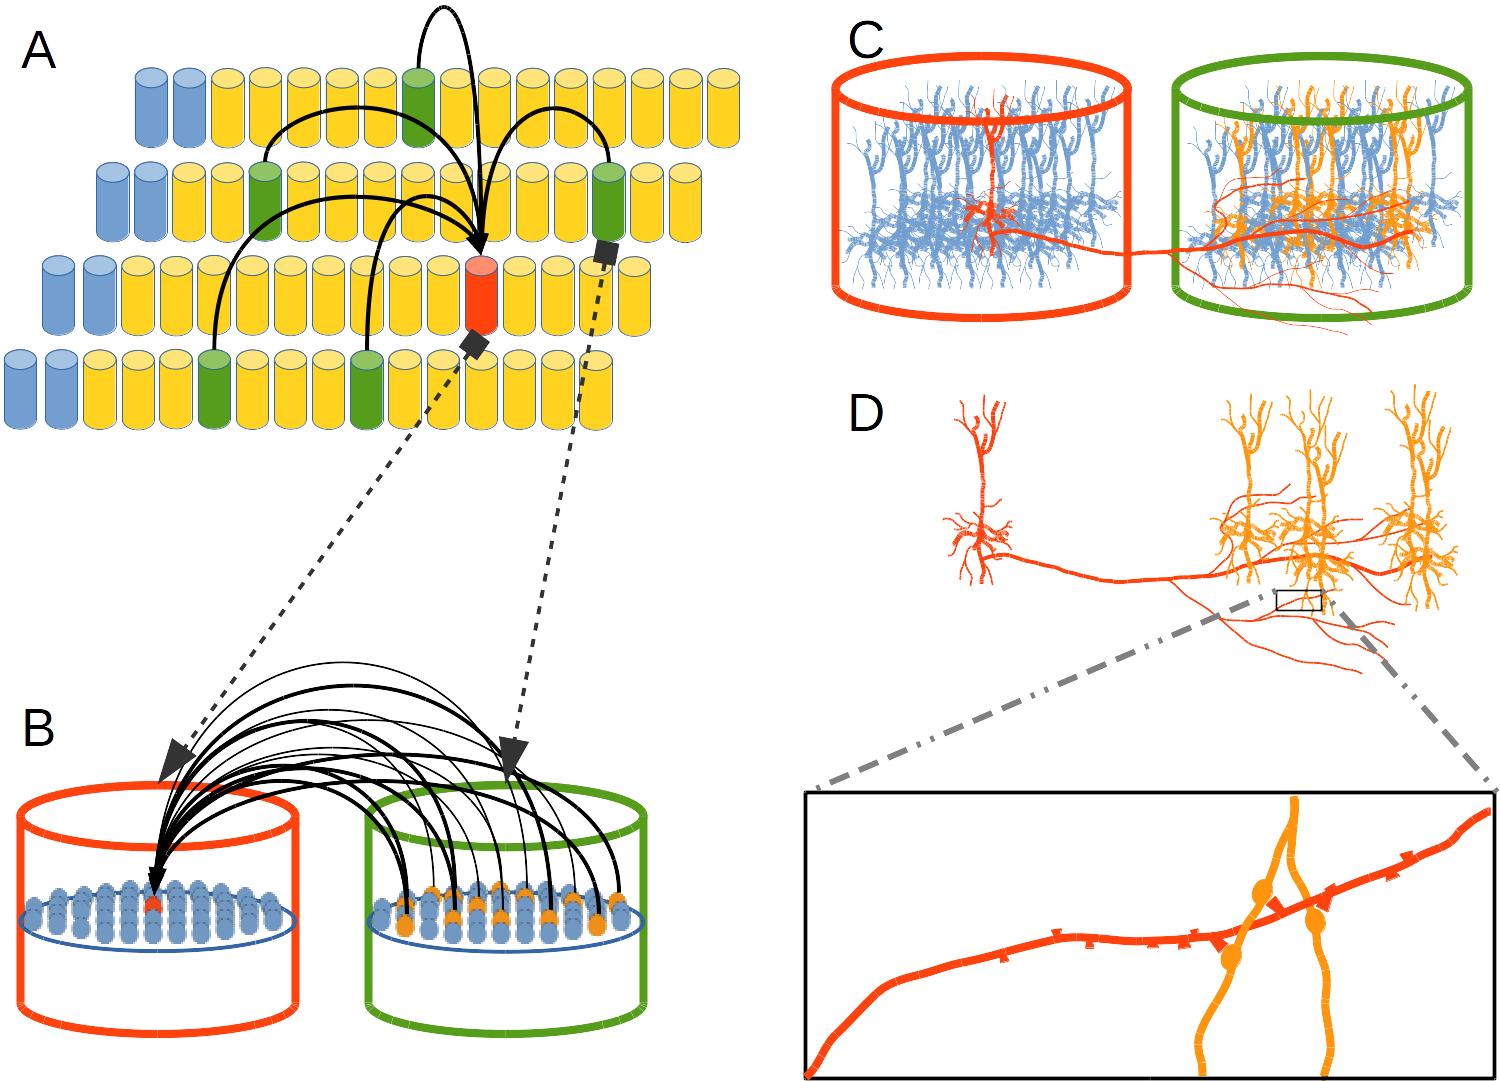
\includegraphics[width=0.7\textwidth]{DistalDendrites.png}
    \caption{Conexiones dendríticas distantes. (A) Ramificaciones dendríticas distantes desde \glspl{cc} dentro del campo receptivo
	    de una \gls{cc} en el \gls{el}. Una rama dendrítica distante entre una \gls{cc} en rojo y una
	    \gls{cc} en verde significa que cada unidad neuronal en la \gls{cc} en rojo está vinculada a un subconjunto diferente
	    de unidades neuronales en la \gls{cc} en verde por medio de conexiones potenciales.
	    (B) Las conexiones potenciales en una rama dendrítica que vinculan una unidad neuronal en la \gls{cc} en rojo
	    con un subconjunto de unidades neuronales en una \gls{cc} en verde. El subconjunto de conexiones potenciales viene de un porcentaje de unidades neuronales
	    dentro de la \gls{cc} en verde. Tal porcentaje es un parámetro ajustable por la \gls{cc}.
	    (C) Una rama dendrítica distante entre una célula piramidal en una \gls{cc} y un 
	    sub-conjunto de células piramidales en una \gls{cc} vecina dentro de su campo receptivo
	    en el \gls{el}.
    (D) La proximidad física de una rama dendrítica desde una célula en rojo a las ramificaciones axonales desde células en amarillo constituyen conexiones potenciales
    que podrían prosperar transformándose en sinapsis establecidas dependiendo de la actividad secuencial entre las células.}
    %\caption{Distal dendrite connections. (A) Distal dendritic branches from neighboring \glspl{cc} inside the receptive field
    %of a \gls{cc} in the \gls{el}. A distal dendritic branch between the red \gls{cc} and a
    %green \gls{cc} means that every neural unit in the red \gls{cc} is linked with a different
    %subset of neural units in the green \gls{cc} by means of potential connections.
    %(B) Potential connections in a dendritic branch which link a neural unit in the red \gls{cc}
    %with a subset of neural units in a green \gls{cc}. The subset of potential connections comes from a percentage of neural units
    %inside the green \gls{cc}. Such percentage is a tunable parameter for the \gls{cc}.
    %(C) A distal dendritic branch between a pyramidal cell in a \gls{cc} and a 
    %sub-set of pyramidal cells in a neighboring \gls{cc} inside its receptive field
    %in the \gls{el}.
    %(D) Physical proximity of a dendritic branch from the red cell to axonal branches from yellow cells constitutes potential connections
    %which could prosper becoming in established synapses depending on the sequential activity among cells.}
    \label{fig:DistalDendrites}
\end{figure}

Tales vínculos en la Fig \ref{fig:DistalDendrites} A, representan ramas dendríticas en el tejido neuronal y nosotros llamamos cada conexión en la Fig. \ref{fig:DistalDendrites} B, conexión potencial. Las conexiones potenciales representan sinapsis en la rama dendrítica. Una unidad celular en la \gls{cc} en rojo termina con tantas ramas dendríticas como \glspl{cc} en verde dentro de su campo receptivo (Fig \ref{fig:DistalDendrites} A.)

%Such links in Fig \ref{fig:DistalDendrites} A, represent dendritic branches in neural tissue and we call each connection in Fig. \ref{fig:DistalDendrites} B, potential connection. Potential connections represent synapses in the dendritic branch. A cell unit inside the red \gls{cc} ends up with as many dendritic branches as green \glspl{cc} inside its receptive field (Fig \ref{fig:DistalDendrites} A.)

El término \emph{conexión potencial} es utilizado porque describe un par de unidades neuronales vinculadas por sus ubicaciones y sus disposiciones dendrítica y axonal en el tejido cortical (Fig. \ref{fig:DistalDendrites} C). Sin embargo, una conectividad efectiva entre tales neuronas dependerá de  su patrón secuencial de activación el que establecerá sinapsis desarrolladas entre ellas. Si dos unidades neuronales--una en rojo y una en amarillo en la Fig. \ref{fig:DistalDendrites} D--están vinculadas por medio de una conexión potencial distante--producida por una sinapsis entre una rama dendrítica distante desde la célula en rojo y una rama axonal desde la célula en amarillo--tal conexión crecerá sólo si hay una activación secuencial de la célula en rojo después de una activación de la célula en amarillo en dos pasos temporales consecutivos. Si tal fenómeno no se repite en el tiempo, tal sinapsis decrecerá con respecto a otras sinapsis en la rama dendrítica en la célula en rojo en la Fig. \ref{fig:DistalDendrites} D. Una activación simultánea en ambas unidades neuronales--la roja y la amarilla en la Fig. \ref{fig:DistalDendrites} D--hará decrecer tal conexión potencial.

%The term \emph{potential connection} is used, because it describes a pair of neural units linked by its physical location and dendritic and axonal disposition in cortical tissue (Fig. \ref{fig:DistalDendrites} C). However, an effective connectivity between such neurons will depend upon their sequential pattern of activation which will establish developed synapses between them. If two neural units--a red one and a yellow one in Fig. \ref{fig:DistalDendrites} D--are linked by means of a distal potential connection--produced by a synapse between a distal dendritic branch from the red one and an axonal branch from the yellow one--such connection will grow only if there is a sequential activation of the red cell after an activation of the yellow cell, in two consecutive time steps. If such phenomenon does not repeat itself over time, such synapse will decrease its strength with respect to other synapses in the dendritic branch in the red cell in Fig. \ref{fig:DistalDendrites} D. A simultaneous activation in both neural units--the red one and the yellow one in Fig. \ref{fig:DistalDendrites} D--will decrease the strength in such potential connection.

Implementamos los mecanismos de plasticidad sináptica dendrítica distante por medio de un algoritmo llamado \gls{dsom} (Alg. \ref{csom_distal_synapses}). El mecanismo de aprendizaje implementado en tal algoritmo simula fenómenos neurofisiológicos como \gls{stdp} y las regulaciones homeostáticas de plasticidad en las sinapsis de las ramas dendríticas distantes. 

%We implemented distal dendritic synaptic plasticity mechanisms by means of an algorithm called \gls{dsom} (Alg. \ref{csom_distal_synapses}). The learning mechanisms implemented on such algorithm simulate neurophysiological phenomena such as \gls{stdp}, and homeostatic regulation plasticity in the synaptic strength regulation in distal dendritic branches.

\begin{algorithm}
	\caption{\texttt{Plasticidad en Sinapsis Distantes}. Este algoritmo implementa los fenómenos de plasticidad y regulación homeostática en sinapsis dendríticas distantes.}
	%\caption{\texttt{Plasticity in Distal Synapses}. This algorithm plasticity and homeostatic phenomenon in distal dendritic synapses.}
\label{csom_distal_synapses}
\begin{algorithmic}[1]
	\FOR{every active \texttt{unit} in this cortical \texttt{column}}
		\FOR{every \texttt{dendrite} in this active \texttt{unit}}
			\STATE {increment all the \texttt{synapses}--in this dendrite--potentially connected to \texttt{units} which were active in the last time step}
		\ENDFOR
	\ENDFOR
	\FOR{every active \texttt{unit} in this cortical \texttt{column}}
		\FOR{every \texttt{dendrite} in this active \texttt{unit}}
			\STATE {decrement all the \texttt{synapses}--in this dendrite--potentially connected to \texttt{units} which are active in this time step}
		\ENDFOR
	\ENDFOR
	\IF{updated \texttt{step} reaches certain value}
		\FOR{every \texttt{unit} in this cortical \texttt{column}}
			\FOR{every \texttt{dendrite} in this \texttt{unit}}
				\IF{the sum of the \texttt{synapses} in this \texttt{dendrite} is greater than one}
					\STATE {normalize all \texttt{synapses} in this \texttt{dendrite}}
				\ENDIF
			\ENDFOR
		\ENDFOR
		\STATE{updated \texttt{step} = 0}
	\ENDIF
	\STATE{updated \texttt{step}++} 
\end{algorithmic}
\end{algorithm}









\subsubsection{Reglas de activación en una \gls{cc} en el \glsfirst{el}}
\label{activation_rules}

En referencia a las reglas de activación de unidades neuronales dentro de una \gls{cc} en el \gls{el}, primero, un grupo de unidades celulares en una \gls{cc} es parcialmente depolarizado por conexiones distantes entre tales unidades neuronales y unidades celulares activadas en el paso temporal previo en el \gls{el}--Fig. \ref{fig:Activation} A. Es decir, unidades neuronales activadas en el paso temporal $t=0$ en el \gls{el}, depolarizarán parcialmente un grupo de unidades neuronales en el paso temporal $t=1$ en tal \gls{cc}, por medio de sinapsis en ramas dendríticas distantes--laterales y apicales--establecidas por aprendizaje en el algoritmo \gls{dsom} (Alg. \ref{csom_distal_synapses}).

%In reference to the activation rules of neural units inside a \gls{cc} in the \gls{el}, first a group of cell units in a \gls{cc} is partially depolarized  by distal connections among such neural units and cell units activated in the previous time step in the \gls{el}--Fig. \ref{fig:Activation} A. That is, neural units activated in time step $t=0$ in the \gls{el}, will partially depolarize a set of neural units in time step $t=1$ in such \gls{cc}, by means of distal--lateral and apical--dendritic branch synapses established by learning in the \gls{dsom} algorithm (Alg. \ref{csom_distal_synapses}).

Segundo, conexiones próximas aferentes desde el \gls{mrstsa} tenderán a depolarizar ciertos clusters de unidades en tal \gls{cc} en el paso temporal $t=1$--Fig. \ref{fig:Activation} B. La depolarización tentativa es producida por las entradas desde el \gls{mrstsa} con sinapsis próximas establecidas por aprendizaje en el algoritmo \gls{ssom} (Alg. \ref{csom_proximal_synapses}). Tal grupo de unidades neuronales son escogidas aleatoriamente desde una distribución discreta cuyas probabilidades son establecidas por el estado de excitación de las entradas aferentes. 

%Second, afferent proximal connections from \gls{mrstsa} will tend to depolarize certain clusters of units in such \gls{cc} in time step $t=1$--Fig. \ref{fig:Activation} B. The tentative depolarization is produced by the inputs from the \gls{mrstsa} with proximal synapses established by learning in the \gls{ssom} algorithm (Alg. \ref{csom_proximal_synapses}). Such group of neural units are randomly chosen from a discrete distribution whose probabilities are established by the state of excitation in afferent inputs.

Si un número suficiente de unidades parcialmente depolarizadas están dentro del conjunto de unidades aferentemente excitadas, tales unidades parcialmente depolarizadas dispararán previamente en el grupo--Fig. \ref{fig:Activation} B izquierda. Tales unidades--que disparan antes--no dejan que unidades vecinas en los clusters excitados disparen, hiper-polarizándolas por medio de conexiones inhibitorias en la columna.

%If a sufficient number of partially depolarized units are in the set of afferently excited units, such partially depolarized units will fire previously in the group--Fig. \ref{fig:Activation} B left. Those units--which fire before--prevent neighboring units in the excited clusters from firing, hyperpolarizing them by means of lateral inhibitory connections in the column.

\begin{figure}[h!]
    \centering
    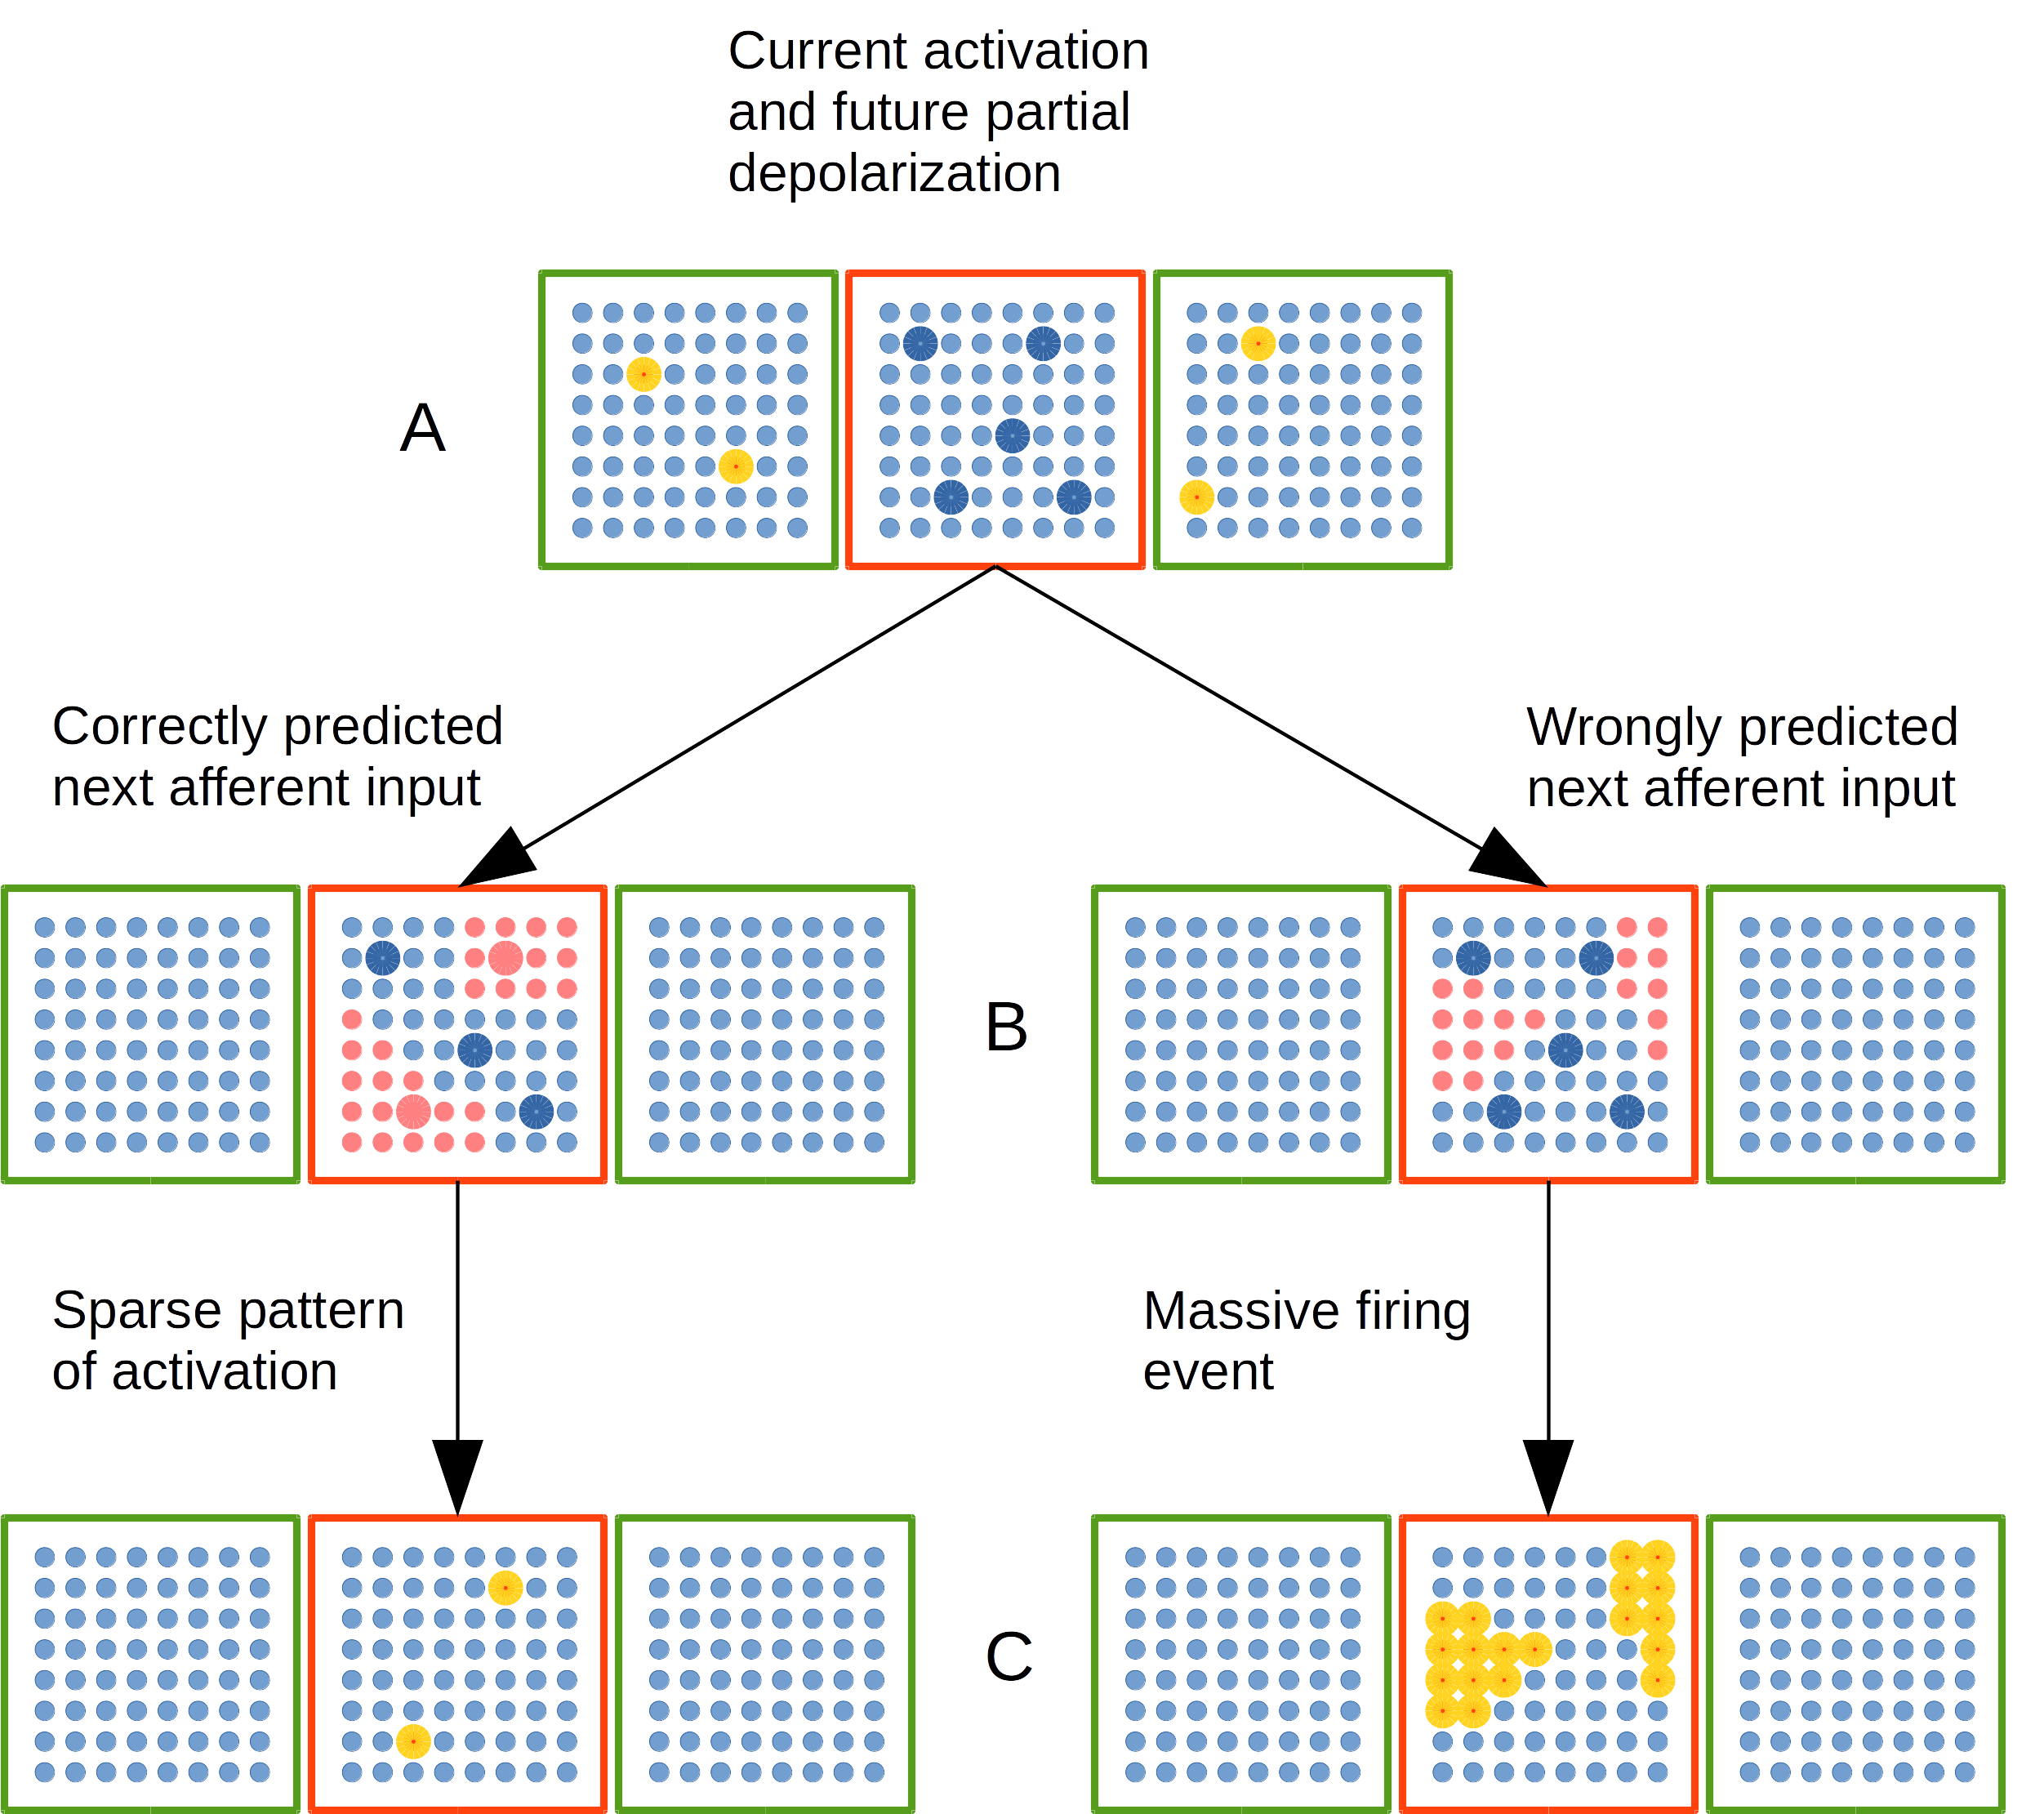
\includegraphics[width=0.7\textwidth]{Activation.png}
    \caption{Activación celular dinámica en una \gls{cc} en el \gls{el}.
    Una columna cortical en rojo está vinculada con dos columnas corticales en verde por medio de dendritas distantes.
    (A) Activación celular en \glspl{cc} en verde--células resaltadas en amarillo--ponen las unidades neuronales
    en la \gls{cc} en rojo en un estado de depolariazación parcial--estado predictivo resaltado en azul.
    (B) Cluster de células neuronales activado por entradas aferentes.
    Izquierda: Una cantidad sustancial de células parcialmente depolarizadas están dentro de los clusters de células aferentemente excitados.
    Derecha: No hay una cantidad sustancial de células parcialmente depolarizadas dentro de los clusters de células aferentemente excitados.
    (C) \gls{cc} con unidades celulares activas resaltadas en amarillo.
    Izquierda: Patrón de activación celular disperso.
    Derecha: Patrón de activación masivo.}
    %\caption{Dynamic cellular activation in a \gls{cc} in the \gls{el}.
    %A red cortical column is linked with two green cortical columns by means of distal dendrites.
    %(A) Cellular activation in green \glspl{cc}--highlighted yellow cells--puts neural units
    %in red \gls{cc} in a partially depolarized--predictive state highlighted in blue.
    %(B) Cluster of neural cells activated by afferent inputs.
    %Left: A substantial amount of partially depolarized cells are in the afferently excited cellular clusters.
    %Right: There is no substantial amount of partially depolarized cells inside afferently excited cellular clusters.
    %(C) \gls{cc} with active cellular units highlighted in yellow.
    %Left: Sparse pattern of cellular activation.
    %Right: Massive pattern of activation.}
    \label{fig:Activation}
\end{figure}

Los estados de depolarización parcial ponen las unidades celulares en un estado predictivo generado por activaciones producidas en el \gls{el} en pasos temporales previos. Es decir, activaciones laterales y apicales en pasos temporales previos constituyen un contexto en el cual las entradas aferentes son recibidas en la actualidad.

%Partial depolarization states put cell units in a predictive state generated by the activations produced in the \gls{el} in previous time steps. That is, lateral and apical activation in previous time steps constitutes a context in which current afferent inputs are received.

Desde el grupo de unidades que tienden a ser depolarizadas por las entradas aferentes actuales desde el \gls{mrstsa}, sólo un sub-grupo reducido de tales unidades pueden disparar en el contexto de la historia de las activaciones en el \gls{el}--Fig. \ref{fig:Activation} C izquierda.

%From the group of units that tend to be depolarized by current afferent inputs from the \gls{mrstsa}, only a reduced sub-set of those units are likely to fire in the previous contextual firing history in the \gls{el}--Fig. \ref{fig:Activation} C left.

En el caso de que no exista contexto, es decir, no hay un número suficiente de unidades dentro de los clusters aferentemente excitados que están parcialmente depolarizadas por activaciones previas--tanto laterales como apicales-- como se muestra en la Fig. \ref{fig:Activation} B derecha, la totalidad de las unidades en los clusters aferentemente excitados se activarán, cubriendo más hipótesis para las entradas aferentes subsecuentes--Fig. \ref{fig:Activation} C derecha.

%In case there is no context, that is, not enough number of the units which tend to be depolarized by afferent inputs is partially depolarized by previous--lateral and apical--activations--Fig. \ref{fig:Activation} B right--, all units in the afferent excited clusters will be active, covering more hypotheses for next inputs--Fig. \ref{fig:Activation} C right.

Tal mecanismo de activación es delineado en el Alg. \ref{csom_activation}. En el Alg. \ref{csom_activation} (Parte 1) se establece un ranking entre unidades neuronales--dentro de una \gls{cc}--en términos de su excitabilidad aferente, dadas las entradas aferentes (líneas 1 y 2). La variable \emph{number of afferently excited units} hace referencia al máximo número de unidades que pueden ser activadas por la entrada aferente en una \gls{cc} y la variable \emph{minimum number of active units} hace referencia al número de unidades que estarán activas en una \gls{cc} si se alcanza una \gls{sdr} como resultado de una predicción óptima (líneas 3 y 4 respectivamente).

%Such activation mechanism is depicted in Alg. \ref{csom_activation}. In Alg. \ref{csom_activation} (Part 1) a ranking is established between neural units--inside a \gls{cc}--in terms of its afferent excitability, given the afferent inputs (lines 1 and 2). The \emph{number of afferently excited units} makes reference to the maximum number of  units that can be activated by the afferent input in a \gls{cc} and \emph{minimum number of active units} makes reference to the number of units that will be active in a \gls{cc} if a \gls{sdr} is achieved as a result of optimal prediction (lines 3 and 4 respectively).

\begin{algorithm}
	\caption{\texttt{Activación de Unidades (Parte 1)}. Este algoritmo establece las reglas de activación en un objeto \gls{csom}.}
\label{csom_activation}
\begin{algorithmic}[1]
	\STATE{\texttt{distances} = given an \texttt{input} vector find the euclidean distance each \texttt{unit} has to such \texttt{input} in the input space from proximal afferent synapses}

	\STATE {\texttt{ranking} = sort indexes from the smallest to the largest \texttt{distances}}

	\STATE{number of afferently excited units = proximal activation percentage*number of units}

	\STATE{minimum number of active units = (1-sparsity)*number of units}

	\IF{randomness is disabled}
		\STATE {excited \texttt{units} = gets the first \emph{number of afferently excited units} elements from \texttt{ranking}}
	\ELSE
		\STATE {excited \texttt{units} = gets \emph{number of afferently excited units} random indexes from \texttt{distances} with probabilities determined by the relative reciprocal of the \texttt{distances} element values}
	\ENDIF

	\FOR{\texttt{unit} = 0 \TO \texttt{unit} = number of units }
		\STATE{auxiliary = 0}
		\FOR{\texttt{dendrite} = 0 \TO \texttt{dendrite} = number of distal dendrites }
			\STATE{\texttt{dendrite} accumulator = 0}
			\FOR{\texttt{active unit} = 0 \TO \texttt{active unit} = number of linked active units}
				\STATE{potential \texttt{index} = find the first coincident index in potential \texttt{connections[dendrite][unit]} with linking \texttt{units[dendrite][active unit]}}
				\IF{there exist coincidence}
					\STATE {\texttt{dendrite} accumulator += dynamic \texttt{synapses[dendrite][unit][\textnormal{potential} index]}}
				\ENDIF
			\ENDFOR
			\IF{\texttt{dendrite} accumulator > 100*DISTAL\_SYNAPTIC\_THRESHOLD}
				\STATE {auxiliary++}
			\ENDIF
		\ENDFOR
		\STATE{total \texttt{responses[unit]} += auxiliary}
	\ENDFOR
	\STATE{updated \texttt{distances} = element wise quotient between \texttt{distances} and total \texttt{responses}}
	\STATE {updated \texttt{ranking} = sort indexes from the smallest to the largest updated \texttt{distances}}

\end{algorithmic}
\end{algorithm}

Si la aleatoriedad está habilitada, una cantidad igual a \emph{number of afferently excited units} de unidades es escogida al azar por medio de una distribución discreta cuyas probabilidades son las excitaciones aferentes de cada unidad. Si la aleatoriedad está deshabilitada, una cantidad igual a \emph{number of afferently excited units} de unidades es escogida desde las primeras unidades en el ranking de las unidades excitadas aferentemente (líneas 5 a 9).

%If randomness is enabled, \emph{number of afferently excited units} amount of units is chosen at random by means of a discrete distribution whose probabilities are the afferent excitation of each unit. If randomness is disabled, \emph{number of afferently excited units} first units are chosen from the ranking of afferently excited units (lines 5 to 9). 

De la línea 10 a la 25 cada unidad neuronal acumula excitación--lateral y apical--distante para determinar su depolarización parcial desde las unidades que estuvieron activas en el paso temporal previo. Para cada unidad neuronal en una \gls{cc}, para cada dendrita distante en tal unidad y para cada unidad activa en tal dendrita distante el algoritmo busca coincidencias entre alguna conexión potencial en tal dendrita distante en la unidad neuronal y la unidad activa en tal dendrita distante. Es decir, en la línea 15, el algoritmo pregunta si existe coincidencia entre alguna conexión potencial en esta dendrita distante dentro de la unidad y la unidad neuronal activada en el paso temporal previo en la \gls{cc} vinculada por tal dendrita distante. Si existe coincidencia, el valor del peso sináptico en tal conexión potencial se acumula en un acumulador de la dendrita. Después de que todas las unidades activas son examinadas para esta dendrita, si el acumulador de la dendrita rebasa cierto umbral, se considera a tal dendrita como activa y la respuesta total de la unidad es incrementada en uno. 

%From line 10 to 25 each neural unit accumulates distal--lateral and apical--excitation in order to determine its partial depolarization from units which were active in the previous time step. For each neural unit in a \gls{cc}, for each distal dendrite in such unit and for each active unit in such distal dendrite the algorithm looks for coincidences between some potential connection in such distal dendrite in the neural unit and the active active unit in such distal dendrite. That is, in line 15, the algorithm ask if there is coincidence between some potential connection in this distal dendrite inside the unit and the neural unit activated in the previous time step in the \gls{cc} linked by such distal dendrite. If there is coincidence, the value of the synaptic weight in such potential connection is accumulated in a dendrite accumulator. After all active units are examined for this dendrite, if the dendrite accumulator is greater than certain threshold, such dendrite is considered active and the total response of the unit is incremented in one.

Cada unidad neuronal termina con un valor de excitación debido a sus dendritas distantes. El vector de distancias de la unidad se divide elemento por elemento por el vector de excitaciones dendríticas para obtener un vector con distancias actualizadas y un ranking actualizado basado en dichas distancias de las unidades (líneas 26 y 27). De esta forma, las unidades con más excitación distante decrementarán más su distancia y serán puestas en una posición más favorable en el ranking a la hora de ser activadas.

%Each neural unit ends up with an excitation value due to its distal dendrites. The unit distances vector is element wise divided by distal dendritic excitations vector to get the updated distances and an updated ranking of the units (lines 26 and 27). In this way, units with more distal excitation will decrease its distance more and will be put in a more favorable place in the ranking in order to be activated.

En el Alg. \ref{csom_activation} (Parte 2), la menor distancia actualizada es hallada en el grupo de unidades excitadas aferentemente. Luego, un conjunto de unidades--dentro del grupo de unidades excitadas aferentemente--con un valor de distancia igual a tal distancia actualizada mínima es identificado. Mientras que el número de unidades identificadas sea menor que \emph{minimum number of active units}, la siguiente distancia actualizada mínima es buscada en el grupo de unidades excitadas aferentemente y un nuevo conjunto de unidades--dentro del grupo de unidades excitadas aferentemente--con tal siguiente distancia actualizada mínima es identificado. Este nuevo grupo es incorporado al grupo previo hasta que el número de unidades en el conjunto acumulado supera a minimum number of active units.

%In Alg. \ref{csom_activation} (Part 2) the minimum updated distance is found in the group of afferently excited units. Then, a set of units--inside the group of afferently excited units--is identified which have such minimum updated distance. While the number of identified units is less than \emph{minimum number of active units}, the next   minimum updated distance is found in the group of afferently excited units and a new set of units--inside the group of afferently excited units--is identified which have such next minimum updated distance. This new set is added to the previous one until the number of units in this accumulative set is greater than or equal to the minimum number of active units.

\begin{algorithm}
\ContinuedFloat
\caption{\texttt{Activación de Unidades (Parte 2)}. Este algoritmo establece las reglas de activación en un objeto \gls{csom}.}
\label{csom_activation}
\begin{algorithmic}[1]
	\STATE{new \texttt{distances} = get the updated \texttt{distances} elements whose indexes are in excited \texttt{units}}
	\STATE{new minimum \texttt{distance} = get the minimum element from new \texttt{distances}}
	\STATE{minimum \texttt{indexes} = get indexes from updated \texttt{distances} vector whose values are equal to new minimum \texttt{distance}}
	\STATE{apt to be \texttt{active} = get the coincident indexes between excited \texttt{units} and minimum \texttt{indexes}}
	\STATE{erase from new \texttt{distances} vector, all the elements whose value is equal to new minimum \texttt{distance}}

	\WHILE{number of elements in apt to be \texttt{active} vector < \emph{minimum number of active units} and new \texttt{distances} has at least one element}
		\STATE{new minimum \texttt{distance} = get the minimum element from new \texttt{distances}}
		\STATE{minimum \texttt{indexes} = get indexes from updated \texttt{distances} vector whose values are equal to new minimum \texttt{distances}}
		\STATE{partial apt to be \texttt{active} = get the coincident indexes between excited \texttt{units} and minimum \texttt{indexes}}
		\STATE{incorporate partial apt to be \texttt{active} elements into apt to be \texttt{active} vector}
		\STATE{erase from new \texttt{distances} vector, all the elements whose value is equal to new minimum \texttt{distance}}
	\ENDWHILE

	\IF{ENABLE\_RANDOM\_BEHAVIOUR}
		\STATE {shuffle apt to be \texttt{active} vector}
	\ENDIF

	\FOR{\texttt{number} = 0 \TO \texttt{number} = number of apt to be \texttt{active} elements }
		\STATE {incorporate to \texttt{output} the excited \texttt{units[\textnormal{apt to be} active[number]]}}
	\ENDFOR

	\RETURN \texttt{output}
\end{algorithmic}
\end{algorithm}

El resultado funcional del Alg. \ref{csom_activation} es que debe haber una cantidad suficiente de unidades neuronales--previa y parcialmente depolarizadas--dentro de los clusters de unidades activados aferentemente a los fines de obtener un patrón de activación \gls{sdr}. De otra forma, la \gls{cc} terminará con un patrón de activación masiva \gls{mfe} en el que más que \emph{minimum number of active units} de unidades estará activa. En el caso de que ocurra un \gls{mfe}, la plasticidad sináptica se modula para reforzar las sinapsis de las unidades activadas durante tal evento.

%The functional result of Alg. \ref{csom_activation} is that there must be a sufficient amount of--partially and previously depolarized-- neural units inside the afferently activated cluster of units in order to get a \gls{sdr} pattern of activation. Otherwise, the \gls{cc} will end up with a massive activation pattern \gls{mfe} in which more than a \emph{minimum number of active units} will be active. In the case of the occurrence of a \gls{mfe}, the synaptic plasticity is modulated in order to form stronger synapses of those neural units activated during such event. 

Cada unidad neuronal en una \gls{cc} establece su estado de depolarización parcial basado en la contribución recibida desde las ramas dendríticas distantes desde conexiones laterales y apicales. Una rama dendrítica contribuirá a la depolarización parcial del soma en tal célula si tal rama dendrítica excede un umbral de activación por medio de la contribución desde sus sinapsis individuales en el contexto de los patrones de activación en el paso temporal previo.

%Each neural unit in a \gls{cc} establishes its state of partial depolarization based on the contribution from distal dendritic branches from lateral and apical connections. A dendritic branch will contribute to the partial depolarization of the soma in such cell only if such dendritic branch exceeds an activation threshold by means of the contribution from its individual synapses in the context of the patterns of activation in the previous time step.

Este mecanismo tiene propiedades secuenciales interesantes \cite{hawkins_2016}, las cuales ya han sido aplicadas en la clasificación de datos secuenciales artificialmente generados \cite{cui_2016}. Nosotros aplicamos tal mecanismo en el algoritmo \gls{dsom} por medio de la adición de sinapsis--en una rama dendrítica--cuyas conexiones están vinculadas con células que estuvieron activas en el paso temporal previo en el \gls{el}. 

%This mechanism has compelling sequential properties \cite{hawkins_2016}, which have already been applied in the classification of artificially generated sequential data \cite{cui_2016}. We apply such mechanism in the \gls{dsom} algorithm by adding the contribution of synapses--in a dendritic branch--whose connections are linked with cells that were active in the previous time step in the \gls{el}.



















\subsection{La Clase \glsfirst{el}}

El \gls{el} es un arreglo multidimensional de \glspl{cc} que obtiene \glspl{sdr} desde las conexiones aferentes próximas desde el \gls{mrstsa}, desde las conexiones laterales distantes desde el mismo \gls{el} y desde las conexiones apicales distantes desde otra \gls{cl} arriba del \gls{el}. En la Fig. \ref{fig:EncoderColumnConnections} se ejemplifica el perfil de la conectividad de una \gls{cc}--en rojo--dentro del \gls{el} el cual es un arreglo bidimensional de \glspl{cc}. Tal \gls{cc} en rojo tiene un campo receptivo aferente sobre el \gls{mrstsa}, un campo receptivo lateral sobre el mismo \gls{el} y un campo receptivo apical sobre otra \gls{cl} encima del \gls{el}. Los campos receptivos se encuentran resaltados en amarillo en la Fig. \ref{fig:EncoderColumnConnections}. La posición de la \gls{cc} en rojo sobre el \gls{mrstsa} y debajo de otra \gls{cl} en la Fig. \ref{fig:EncoderColumnConnections} determina sus centros correspondientes sobre el el arreglo \gls{mrstsa} y sobre la \gls{cl} encima del \gls{el}. Cada campo receptivo tiene un tamaño que se desarrolla alrededor de los centros de la \gls{cc}. En el caso mostrado en la Fig. \ref{fig:EncoderColumnConnections} los campos receptivos tienen la propiedad wraparound. Esta propiedad permite al campo receptivo extenderse más allá de los límites físicos impuestos por los lados y/o esquinas, utilizando espacio en los lados y esquinas opuestas en la capa. La propiedad de wraparound así como el tamaño de los campos receptivos son parámetros ajustables en el \gls{el}. Si la propiedad wraparound está deshabilitada, los centros de las \glspl{cc} que se encuentran cerca de los lados y/o esquinas en la capa, recibirán una superficie menor de campo receptivo. Los campos receptivos de las \glspl{cc} determinan el alcance de la conectividad de tal \gls{cc} en las diferentes capas del modelo. Dentro de cada campo receptivo, hay algunos módulos verdes en la Fig. \ref{fig:EncoderColumnConnections} que representan los elementos realmente vinculados con la \gls{cc} en rojo en tales campos receptivos. Cada conjunto de elementos en verde constituye cierto porcentaje desde el número total de elementos en el campo receptivo correspondiente. Tal porcentaje, también es un parámetro ajustable en el \gls{el}. 

%The \gls{el} is a multidimensional array of \glspl{cc} that obtains \glspl{sdr} from proximal afferent connections from the \gls{mrstsa}, from distal lateral connections from the same \gls{el} and from distal apical connections from other \gls{cl} above the \gls{el}. In Fig. \ref{fig:EncoderColumnConnections} we exemplify the connectivity profile of a \gls{cc}--in red--inside the \gls{el} which is a bi-dimensional array of \glspl{cc}. Such red \gls{cc} has an afferent receptive field on the \gls{mrstsa}, a lateral receptive field on the same \gls{el} and an apical receptive field on another \gls{cl} above the \gls{el}. Receptive fields are highlighted in yellow in Fig. \ref{fig:EncoderColumnConnections}. The position of the red \gls{cc} above the \gls{mrstsa} and below the other \gls{cl} in Fig. \ref{fig:EncoderColumnConnections} determines its corresponding centers on the \gls{mrstsa} array and on the \gls{cl} above the \gls{el}. Each receptive field has a size which is developed about its \gls{cc} corresponding centers. In the case depicted in Fig. \ref{fig:EncoderColumnConnections} receptive fields have wraparound property. This property allows receptive fields to extend beyond the physical limits imposed by sides and/or corners, using space on opposite sides and corners in the layers. Wraparound property as well as size of the receptive fields are tunable parameters in the \gls{el}. If wraparound property is disabled, \glspl{cc} centers near sides and corners in the layer will receive less receptive field surface. \gls{cc} receptive fields determine the connectivity scope of such \gls{cc} in the different layers of the model. Inside each receptive field, there are some green modules in Fig. \ref{fig:EncoderColumnConnections} which represent elements which are really connected to the red \gls{cc} in such receptive fields. Each set of green elements constitutes certain percentage from the total number of elements in its corresponding receptive field. Such percentage is also a tunable parameter in the \gls{el}. 

\begin{figure}[h!]
    \centering
    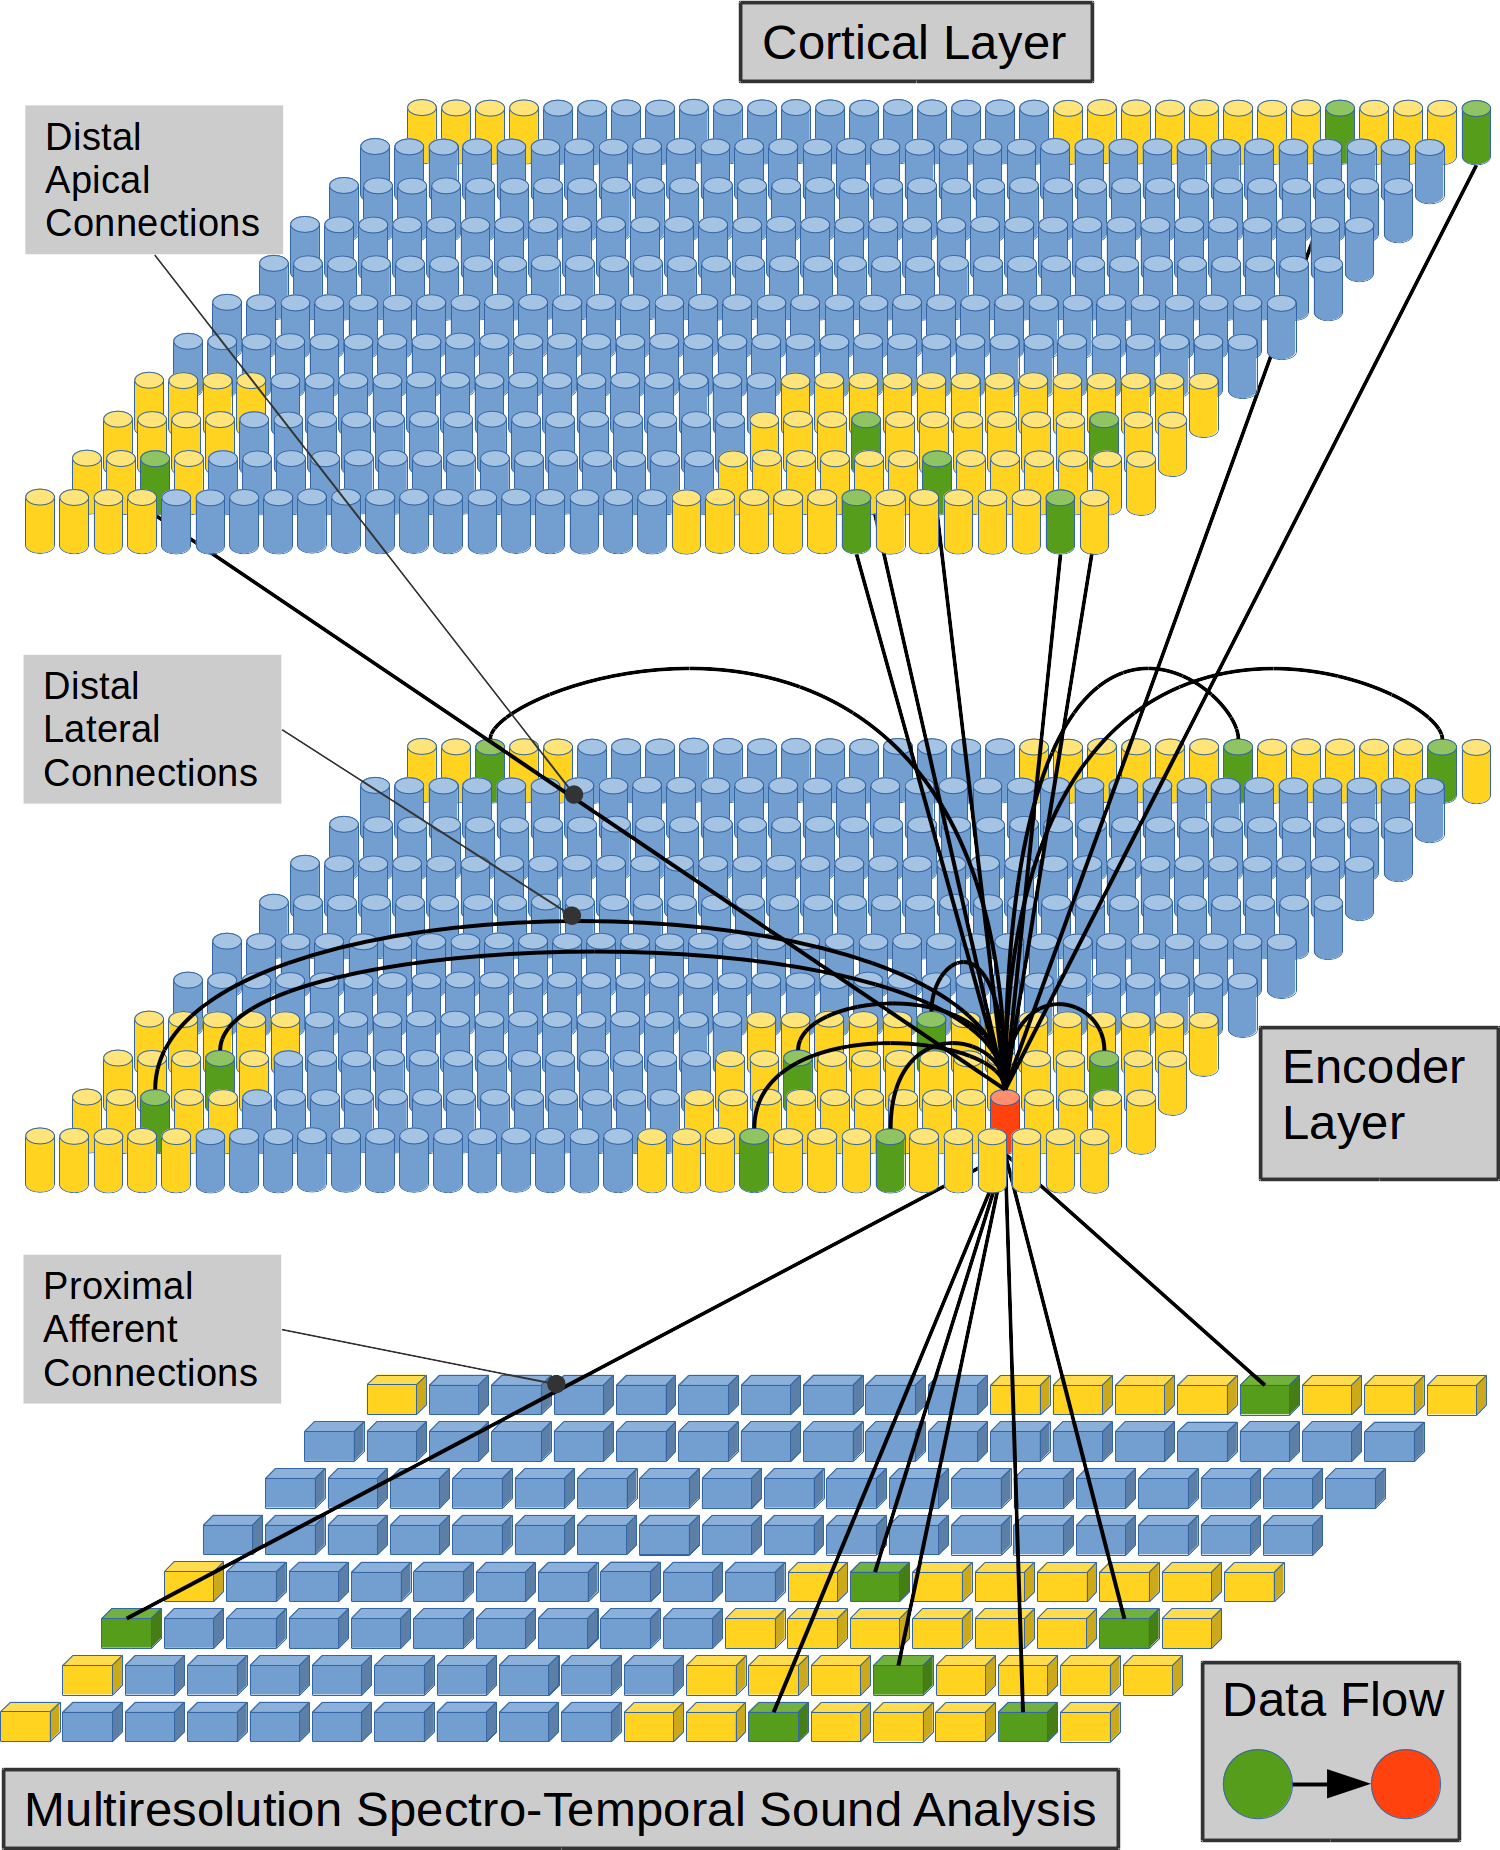
\includegraphics[width=0.6\textwidth]{EncoderColumnConnections.png}
    \caption{Esquema de conexión para una columna cortical en el Encoder Layer.
    Cada cilindro en el \gls{el} y en la \gls{cl} representa una \gls{cc} en el tejido neuronal.
    Cada prisma en el \gls{mrstsa} representa una variable con un número real.
    Esta es una visualización de una \gls{cc} (en rojo) y sus tres campos receptivos (en amarillo).
    El campo receptivo de una \gls{cc} es un arreglo que define un conjunto de \glspl{cc}
    con el que tal columna puede estar conectada.
    El campo receptivo de una \gls{cc} sobre el \gls{mrstsa} determina un arreglo de variables en valores reales
    con el cual tal columna puede estar conectada.
    Un subconjunto de \gls{cc} en un campo receptivo (en verde) representa las \glspl{cc} que están realmente
    conectadas con la \gls{cc} en rojo. Un escenario similar se puede describir para los prismas verdes sobre
    el \gls{mrstsa}.
    El tamaño, la propiedad wrap-around y el porcentaje de vínculos establecidos (en verde) dentro de un campo receptivo son parámetros ajustables para el modelo.
    En este trabajo, se han implementado sólo conexiones laterales ya que en la implementación actual no hay una capa cortical superior al \gls{el} desde la cual
    traer conexiones apicales.}
    %\caption{Connection scheme for a cortical column in the Encoder Layer.
    %Each cylinder in the \gls{el} and in the \gls{cl} represents a \gls{cc} in neural tissue.
    %Each prism in the \gls{mrstsa} represents a real valued variable.
    %This is a visualization of a \gls{cc} (in red) and its three receptive fields (in yellow).
    %The receptive field of a \gls{cc} is an array that defines a set of \glspl{cc}
    %with which such column could be connected.
    %The receptive field of a \gls{cc} on the \gls{mrstsa} determines an array of real valued variables
    %with which such column could be connected.
    %A subset of \glspl{cc} in a receptive field (in green) represents the \glspl{cc} that are really
    %connected with the \gls{cc} in red. A similar scenario could be described for the green prisms on
    %the \gls{mrstsa}.
    %The size, wrap-around property and percentage of established links (in green) inside a receptive field are tunable parameters for the model.
    %In this work, only lateral connections have been implemented since in the current implementation there are no upper cortical layers from which
    %to bring apical connections.}
    \label{fig:EncoderColumnConnections}
\end{figure}

Los módulos individuales en el \gls{mrstsa} son muy diferentes a los módulos individuales en el \gls{el} o en la \gls{cl} arriba. Los módulos individuales en el \gls{mrstsa} son variables escalares--números reales--(sección \ref{mrstsa}) mientras que los módulos individuales sobre el \gls{el} y la \gls{cl} son \glspl{cc}. Esta circunstancia determina que las conexiones próximas aferentes son muy diferentes de las conexiones distantes--laterales y/o apicales. Mientras que las conexiones aferentes próximas son pesos sinapticos individuales (sección \ref{proximal_dendrites}), las conexiones distantes son ramas dendríticas complejas (sección \ref{distal_dendrites}).

%Individual modules on the \gls{mrstsa} are very different from individual modules on the \gls{el} or on the \gls{cl} above. Individual modules on the \gls{mrstsa} are scalar--real valued--variables (section \ref{mrstsa}) while individual modules on the \gls{el} and \gls{cl} are \glspl{cc}. This circumstance determines that proximal afferent connections are very different from distal--lateral and/or apical--connections. While proximal afferent connections are individual synaptic weights (section \ref{proximal_dendrites}), distal connections are complex dendritic branches (section \ref{distal_dendrites}). 

La clase \gls{el} configura toda la conectividad para cada \gls{cc}, esto es, determina los elementos aleatorios desde el \gls{mrstsa}--dentro del campo receptivo en tal \gls{cc}--los cuales serán vinculados con la \gls{cc}, determina el conjunto aleatorio de conexiones potenciales para cada elemento en cada dendrita distante. Toda esta configuración de conectividad para cada \gls{cc} se guarda después de un procedimiento inicial de construcción de un objeto de clase \gls{el}.

%The \gls{el} class configures all the connectivity for each \gls{cc}, that is, determines the random elements from the \gls{mrstsa}--inside the receptive field of such \gls{cc}--which will be linked with the \gls{cc}, determines the random set of potential connections to each element in each distal dendrite. All this connectivity configurations for each \gls{cc} is saved after an initial procedure of construction of a \gls{el} object. 

En cada paso temporal, el \gls{el} reúne la información desde las conexiones aferente, lateral y apical y hace dicha información disponible para cada \gls{cc}. En el algoritmo \gls{som}, cada vector de entrada tiene que estar completamente determinado. En nuestro caso, algunas entradas desde el \gls{mrstsa} podrían ser nulas, y cada vector de entrada podría no tener la información de cada una de sus componentes disponible. Incorporamos un mecanismo estocástico al \gls{el} para lidiar con tal situación. Hicimos que cada conexión aferente aprenda los límites estadísticos de su entrada correspondiente. Establecemos márgenes mínimo-máximo para cada conexión próxima en el \gls{el}. Tales márgenes tienen consistencia con la distribución estadística en la historia de sus entradas correspondientes. Cuando una entrada aferente está indeterminada, en un contexto en el cual algunas entradas aferentes cuentan con información disponible, el \gls{el} escoge el valor en las entradas indeterminadas  de manera aleatoria entre los límites aprendidos para tal entrada.

%In each time step, the \gls{el} gathers the information from afferent, lateral and apical connections and makes this information available for each \gls{cc}. In the \gls{som} algorithm, each input vector has to be completely determined. In our case, some inputs from the \gls{mrstsa} could be null, and each input vector could not have the information of each of its components available. We incorporated a stochastic mechanism in the \gls{el} in order to deal with such situation. We made each afferent connection to learn statistical boundaries from its corresponding input. We establish a minimum-maximum margin in each proximal connection in the \gls{el}. Such margin is consistent with the statistical distribution in the history of its corresponding input. When an afferent input is undetermined, in a context in which some afferent inputs have available information, the \gls{el} chooses the value in the undetermined input randomly between the boundaries learned for such input.








%\subsubsection{Paralelización del \glsfirst{el}}

%Paralelizamos la clase \gls{el} por medio del paradigma híbrido \gls{mpi}+\gls{omp}. Distribuimos \glspl{csom} entre \gls{mpi} ranks como un mazo de cartas es distribuido entre diferentes jugadores. Cada \gls{mpi} rank termina con uno o más \glspl{csom} y los \glspl{csom} en cada rank son distribuidos entre diferentes hilos \gls{omp} (Fig. \ref{fig:EncoderParallelization} A y B respectivamente). La información entre \gls{mpi} ranks debe ser transferida en cada paso temporal. Reunimos toda la información correspondiente a los \glspl{csom} en cada rank y luego utilizamos la función \gls{mpi} Bcast  para transmitir tal información utilizando un protocolo de comunicación especial por medio del cual especificamos los límites en la información correspondiente a cada \gls{csom} (Fig. \ref{fig:EncoderParallelization} C). Por medio de esta estratégia cada \gls{mpi} rank tiene que llamar a \gls{mpi} Bcast sólo una vez a los fines de transmitir sus datos. El \gls{el} utiliza un sistema de archivo en paralelo para guardar su estado en formatos Matlab/Octave (Fig. \ref{fig:EncoderParallelization} D). Cada \gls{mpi} rank reune todos los datos correspondientes a sus \glspl{csom} en el \gls{el} y comunica la parte del archivo que utilizará a los otros \gls{mpi} ranks para guardar los datos sin interferir  con otros ranks en el ambiente \gls{mpi}. Luego, cada \gls{mpi} rank guarda todos sus datos con una única llamada a \gls{mpi} Write.

%%We parallelize the \gls{el} class by means of a hybrid \gls{mpi}+\gls{omp} paradigm. We distribute \glspl{csom} among \gls{mpi} ranks as a deck of cards is distributed among different players. Each \gls{mpi} rank ends up with one or more \glspl{csom} and the \glspl{csom} in each rank are distributed among different \gls{omp} threads (Fig. \ref{fig:EncoderParallelization} A and B respectively). Information among \gls{mpi} ranks must be transferred in each time step. We gather all the information corresponding to the \glspl{csom} in each rank and then use \gls{mpi} Bcast function to transmit such information using a special comunication protocol by means of which we specify the boundaries in the information corresponding to each \gls{csom}(Fig. \ref{fig:EncoderParallelization} C). By means of this strategy each MPI rank has to call \gls{mpi} Bcast just once in order to transmit its data. The \gls{el} uses \gls{mpi} I/O parallel file system to save its status in Matlab/Octave format (Fig. \ref{fig:EncoderParallelization} D). Each \gls{mpi} rank gathers all the data corresponding to its \glspl{csom} in the \gls{el} and communicates the part of the file it will use to the other \gls{mpi} ranks, in order to store the data without interfering with the other ranks in the \gls{mpi} environment. Then, each \gls{mpi} rank saves all its data with a unique call to \gls{mpi} Write. 

%\begin{figure}[h!]
    %\centering
    %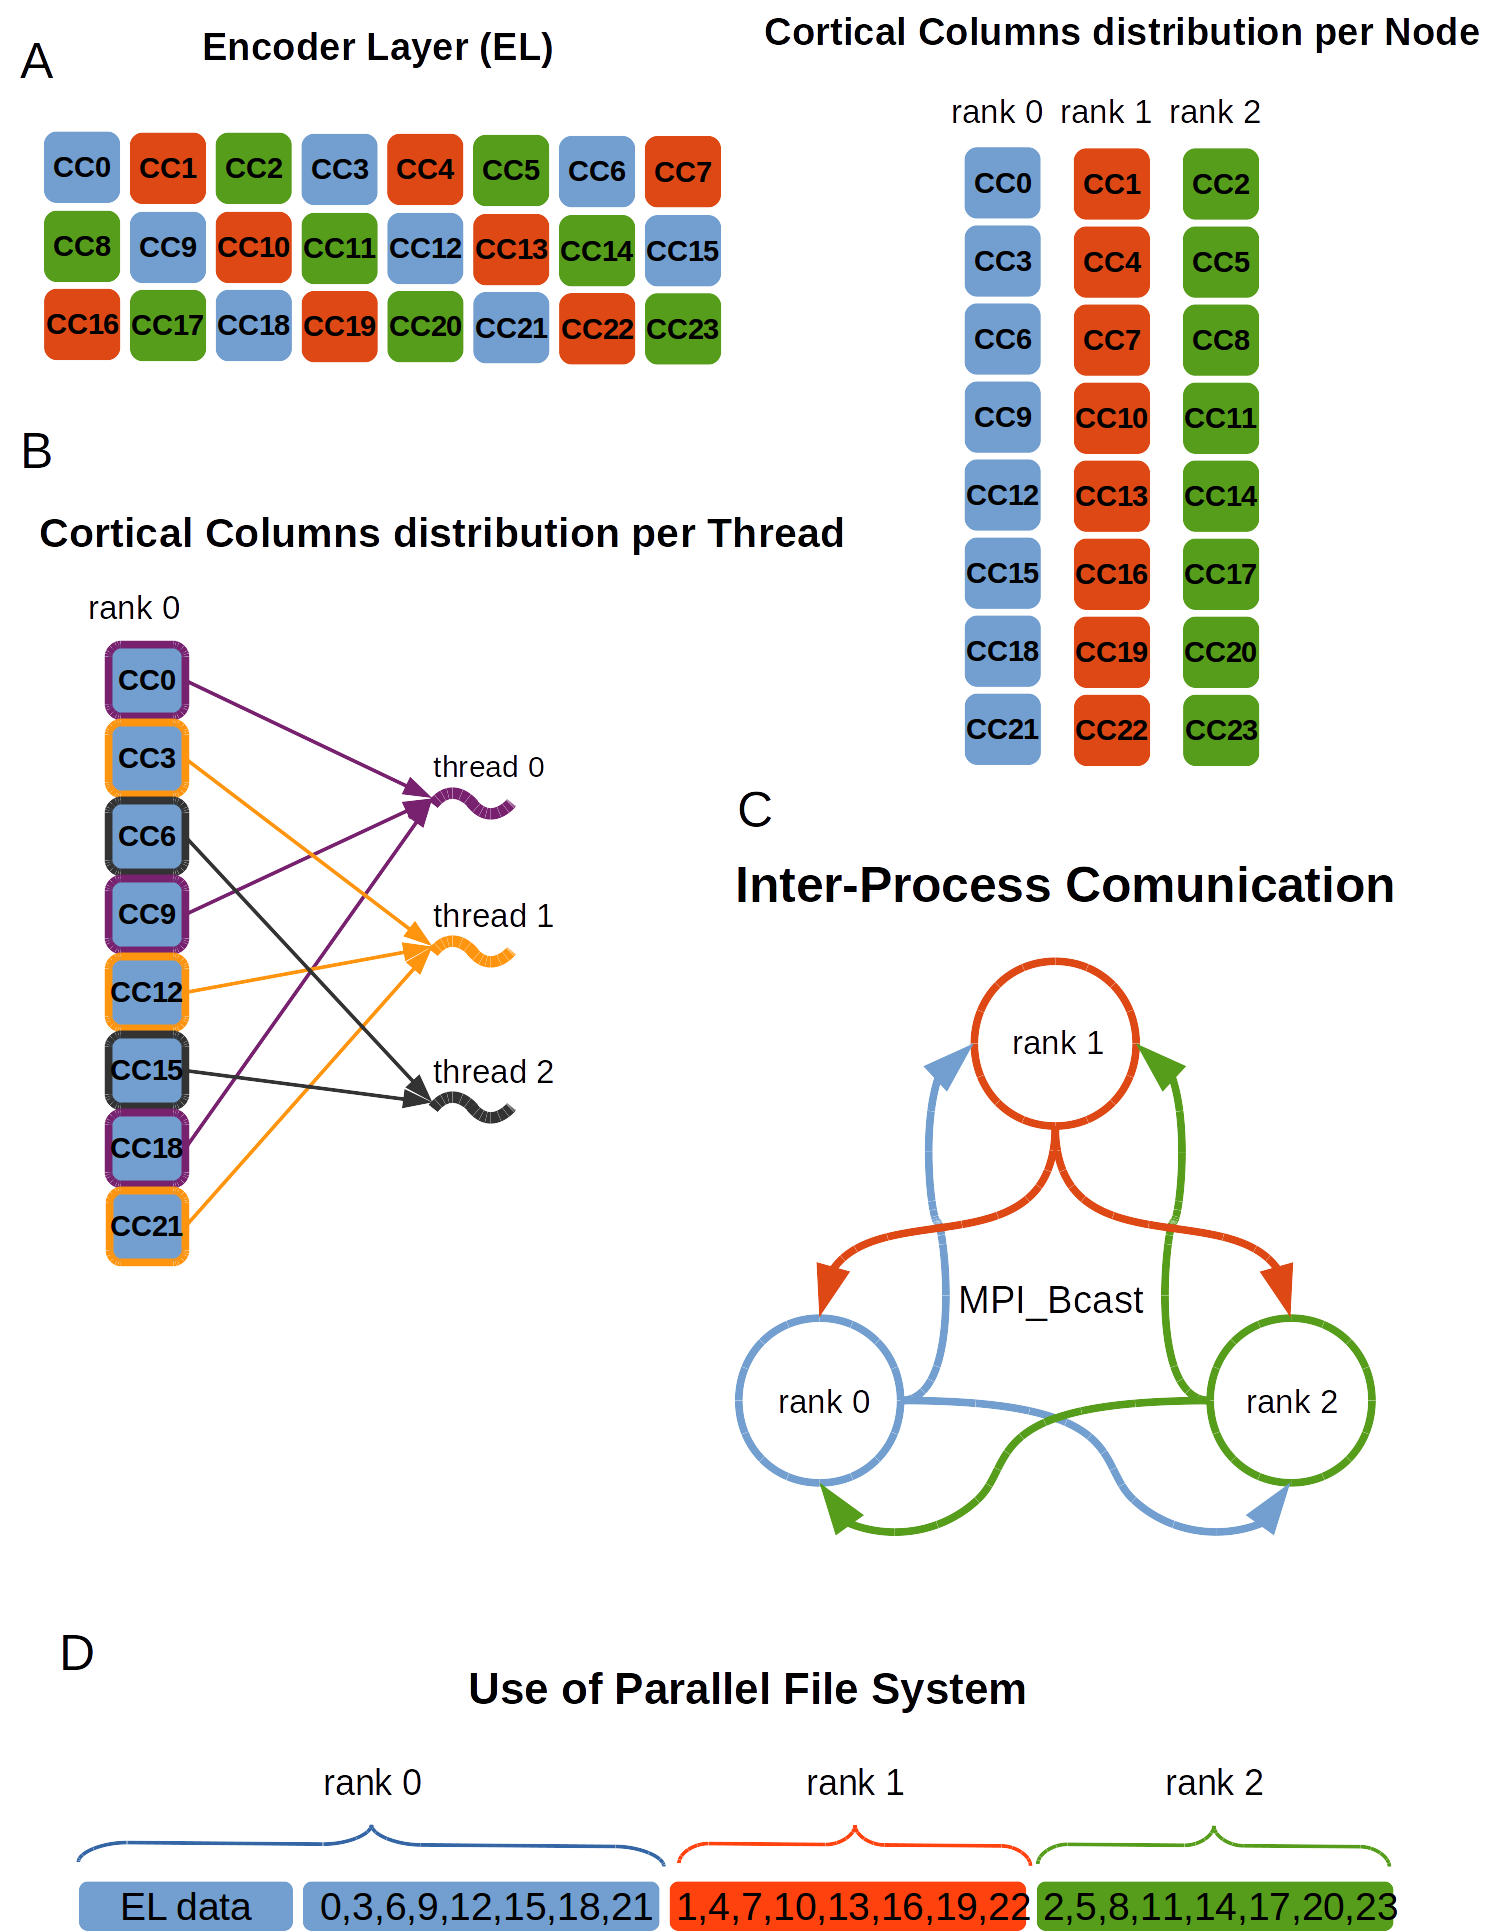
\includegraphics[width=0.7\textwidth]{EncoderParallelization.png}
    %\caption{Paralelización \gls{mpi}+\gls{omp} del \glsfirst{el}. (A) Distribución de objetos \gls{csom} en un \gls{el} con
	    %3 por 8 (24) \glspl{cc} entre tres \gls{mpi} ranks con tres hilos \gls{omp} por rank.
    %Ciertos ranks podrían hacerse cargo de un número diferente de
    %\glspl{csom} dependiendo del número de \gls{mpi} ranks así como también del número de \glspl{cc} en el \gls{el}.
    %(B) Cada \gls{mpi} rank distribuye sus \glspl{csom} entre diferentes hilos de la misma manera.
    %(C) \gls{mpi} \gls{ipc} entre diferentes ranks. El \gls{ipc} se lleva a cabo en cada paso temporal ya que cada \gls{mpi} rank 
    %requiere la salida completa del \gls{el} en cada paso temporal.
    %Cada \gls{mpi} rank difunde la información correspondiente a sus \glspl{cc} a los otros ranks en el ambiente \gls{mpi}.
    %(D) Distribución de la información del \gls{el} en un archivo para guardar su estado.
    %Cada \gls{mpi} rank pone los datos formateados correspondientes a sus \glspl{csom} en una clase template \gls{stl} stringstream.
    %El Rank 0 también se hace cargo de la estructura, conectividad y parámetros del \gls{el}.
    %Una vez que cada rank tiene su stringstream con los datos formateados, comunica su file view a los otros ranks.
    %Luego, cada rank escribe su flujo de bytes en paralelo sin interferir con los otros ranks en el ambiente \gls{mpi}.
    %Un \gls{el} con un número diferente de ranks puede cargar el mismo archivo sin afectar el resultado final.
    %Cada rank en el nuevo \gls{el} carga el archivo completo en una clase template \gls{stl} stringstream y luego toma la información que le concierne de tal estructura.}
    %%\caption{\glsfirst{el} \gls{mpi}+\gls{omp} parallelization. (A) Distribution of \gls{csom} objects in an \gls{el} with
    %%3 by 8 (24) \glspl{cc} among three \gls{mpi} ranks with three \gls{omp} threads per rank.
    %%Certain ranks could take care of a different number of
    %%\glspl{csom} depending on the number of \gls{mpi} ranks as well as the number of \glspl{cc} in the \gls{el}.
    %%(B) Each \gls{mpi} rank distributes its \glspl{csom} among different threads in the same fashion.
    %%(C) \gls{mpi} \gls{ipc} among different ranks. \gls{ipc} is carried out at each time step since each \gls{mpi} rank 
    %%requires the complete \gls{el} output at each time step.
    %%Each \gls{mpi} rank broadcasts the information corresponding to its \glspl{cc} to the other ranks in the \gls{mpi}
    %%environment.
    %%(D) \gls{el} information distribution in a file to save its status.
    %%Each \gls{mpi} rank puts the formated data corresponding to its \glspl{csom} in a \gls{stl} stringstream class template.
    %%Rank 0 also takes care of the \gls{el} structure, connectivity and parameters.
    %%Once each rank has its stringstream with the formated data, it communicates its file view to the other ranks.
    %%Then each rank writes its stream of bytes in parallel without interfering with other ranks in the \gls{mpi} environment.
    %%An \gls{el} with a different number of ranks can load the same file without affecting the final results.
    %%Each rank in the new \gls{el} loads the complete file in a \gls{stl} stringstream class template and then takes the
    %%informations that concern it from such structure.}
    %\label{fig:EncoderParallelization}
%\end{figure}






%\subsubsection{Herencia y Estructura Composicional Jerárquica del \glsfirst{el}}

%Implementamos nuestros algoritmos con el estandard \CC14 utilizando el paradigma de programación orientada a objetos o \gls{oop} en un conjunto de clases interrelacionadas por herencia y composición. Implementamos conectividad aferente próxima y distante intercolumnar así como los márgenes mínimos/máximos en los pesos sinápticos aferentes en  la clase \glsfirst{el}. Configuramos tal clase como una composición de objetos de la clase \glsfirst{csom}. El miembro principal de la clase \gls{el} es un vector \gls{stl} con objetos \gls{csom}. Un diagrama completo de la estructura composicional y de herencia jerárquica de la implementación se muestra en la Fig. \ref{fig:InheritanceComposition}.

%%We implement our algorithms in standard \CC14 using the \gls{oop} paradigm in a set of classes interrelated by inheritance and composition. We implement proximal afferent and distal inter-columnar connectivity   as well as minimum-maximum margins in afferent synaptic weights in the \glsfirst{el} class. We configure such class as a composition of objects of class \glsfirst{csom}. The main member in the \gls{el} class is a \gls{stl} vector of \gls{csom} objects. A complete diagram of the hierarchical inheritance and compositional structure of the implementation can be seen in Fig. \ref{fig:InheritanceComposition}.

%\begin{figure}[h!]
    %\centering
    %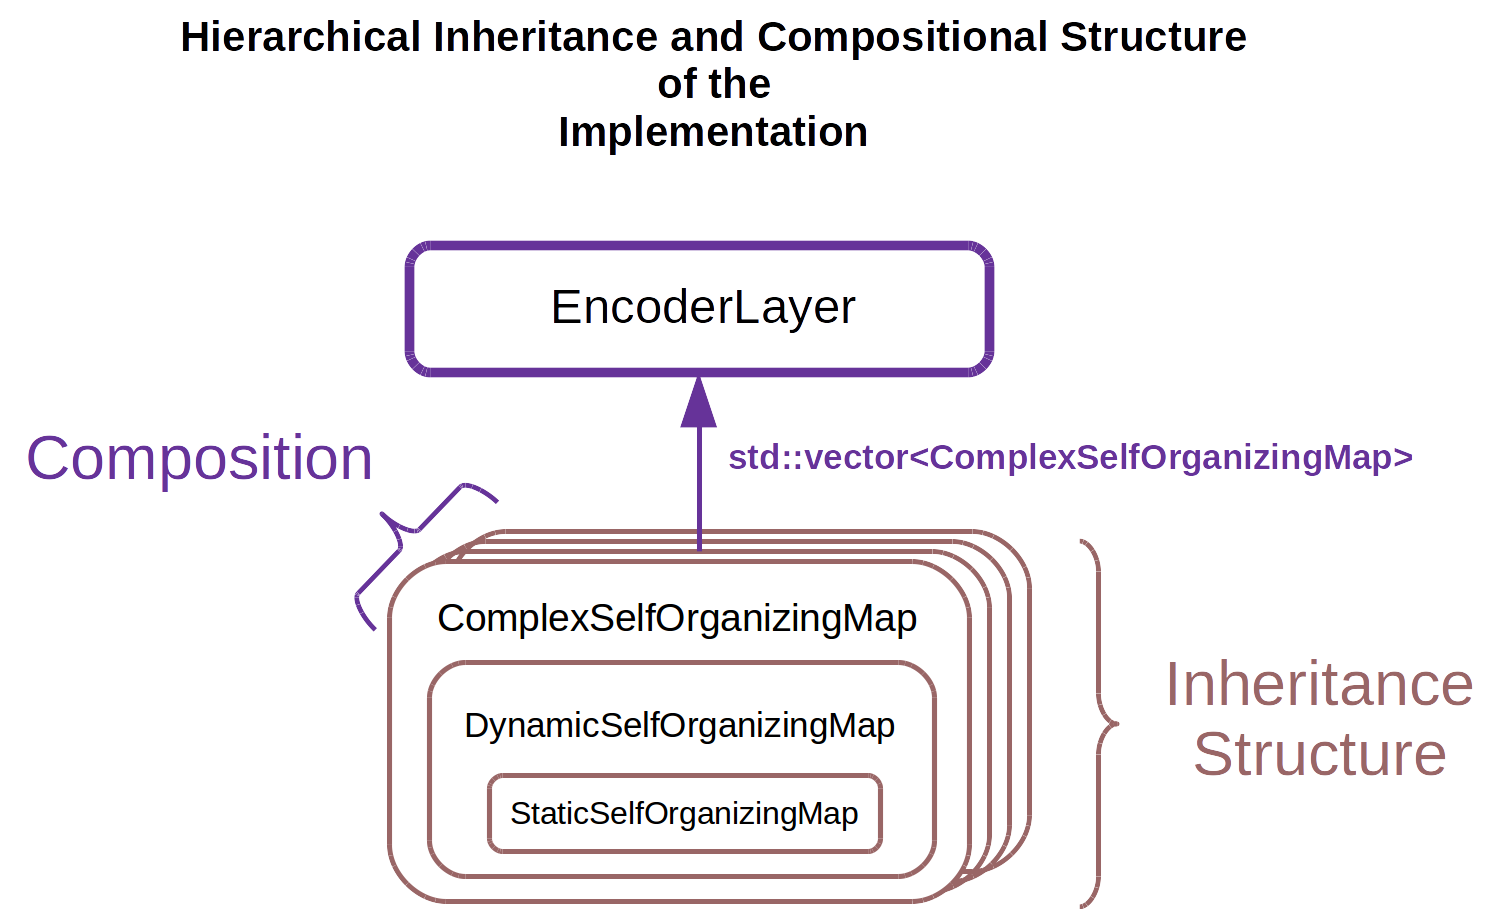
\includegraphics[width=0.8\textwidth]{InheritanceComposition.png}
    %\caption{Estructura Hereditaria y Composicional Jerárquica de la implementación del modelo.
    %La clase \glsfirst{csom} hereda desde la clase \glsfirst{dsom} la cual hereda desde \glsfirst{ssom}.
    %El \glsfirst{el} está formado por la composición de un conjunto de \glspl{csom} agrupados
    %en un contenedor std::vector \glsfirst{stl}.}
    %%\caption{Hierarchical Inheritance and Compositional Structure of the Model Implementation.
    %%\glsfirst{csom} inherits from \glsfirst{dsom} which inherits from \glsfirst{ssom}.
    %%The \glsfirst{el} is formed by the composition of a set of \glspl{csom} gathered
    %%in a std::vector \glsfirst{stl} container.}
    %\label{fig:InheritanceComposition}
%\end{figure}










%\section{Clasificación Fonética, un Caso de Estudio}

%Proponemos un modelo computacional llamado \gls{cstm}, que consiste de dos partes: El \gls{el} y el \gls{mrstsa}.  

%%We propose a computational approach called \gls{cstm}, which consists of two parts: The \gls{el} and the \gls{mrstsa}.  

%EL algoritmo \gls{mrstsa}, el cual procesa las ondas de sonido para alimentar la entrada al \gls{el}, es una técnica inspirada en Chi T. et al. \cite{chi_2005}. En su trabajo, hallazgos experimentales acumulados desde el sistema auditivo central se explotaron demostrando su aplicación en la evaluación objetiva de la inteligibilidad del habla. En el presente trabajo, debido a que promovemos la incorporación parsimoniosa de propiedades neurofisiológicas--principalmente centradas en las características de la corteza--seguimos las líneas principales en la implementación de la sección cortical de tal modelo.

%%The algorithm \gls{mrstsa}, which processes the sound waves to feed inputs to the \gls{el}, is a technique inspired by Chi T. et al. \cite{chi_2005}. In their work, accumulating experimental findings from the central auditory system were exploited demonstrating its applications in the objective evaluation of speech intelligibility. In the present work, since we prompt a parsimonious incorporation of neurophysiological properties--mainly centered in cortical features--we followed the main guidelines in the implementation of the cortical section of such model.

%El \gls{el} convierte un arreglo multidimensional de números reales en un \gls{sdr} multidimensional. Esta etapa está compuesta por un conjunto de \glspl{som} \cite{kohonen_2082, Kohonen:1989:SAM:69371} e incorpora fenómenos neurofisiológicos como la organización columnar, la formación aferente espontánea micro-columnar, las arborizaciones dendríticas próximas y distantes, la interacción intercolumnar lateral por medio de activaciones de ramas dendríticas independientes con receptores \gls{nmda}, los \glspl{mfe} con adaptación a estímulos contextuales, inhibición intracolumnar lateral próxima, \gls{ltp}, \gls{ltd}, \gls{stdp} y regulaciones homeostáticas sinaptica.

%%The \gls{el} converts a multidimensional array of real numbers into a multidimensional \gls{sdr}. This stage is composed by a set of \glspl{som} \cite{kohonen_2082, Kohonen:1989:SAM:69371} and incorporates neurophysiological phenomena such as columnar organization, afferent spontaneous micro-columnar formation, proximal and distal dendritic arborization, lateral intercolumn interaction by means of independent dendritic \gls{nmda} branch activations, \glspl{mfe} with contextual stimulus adaptation, proximal lateral intracolumn inhibition, \gls{ltp}, \gls{ltd}, \gls{stdp} and distal synaptic homeostatic regulations.

%En el presente trabajo, estudiamos el nivel de invarianza en las características fonéticas abstraídas por el \gls{el}, por medio de la comparación de tales representaciones con características auditivas espectro-temporales de múltiple resolución devueltas por el algoritmo \gls{mrstsa}. A tal efecto, evaluamos las características devueltas por cada algoritmo en diferentes tareas de clasificación de palabras. Para probar el desempeño en clasificación de palabras en cada algoritmo, utilizamos la técnica \gls{svm} con la configuración experimental delineada en la Fig. \ref{fig:Experiment}.

%%In the present work, we studied the level of invariance in the phonetic features abstracted by the \gls{el}, by means of comparing such representations with the multiresolution spectro-temporal auditory features returned by the \gls{mrstsa} algorithm. To this end, we evaluated the features returned by each algorithm in different word classification tasks. In order to asses the word classification performance in each algorithm, we used \gls{svm} technique with the experimental setup depicted in Fig. \ref{fig:Experiment}.

%\begin{figure}[h!]
    %\centering
    %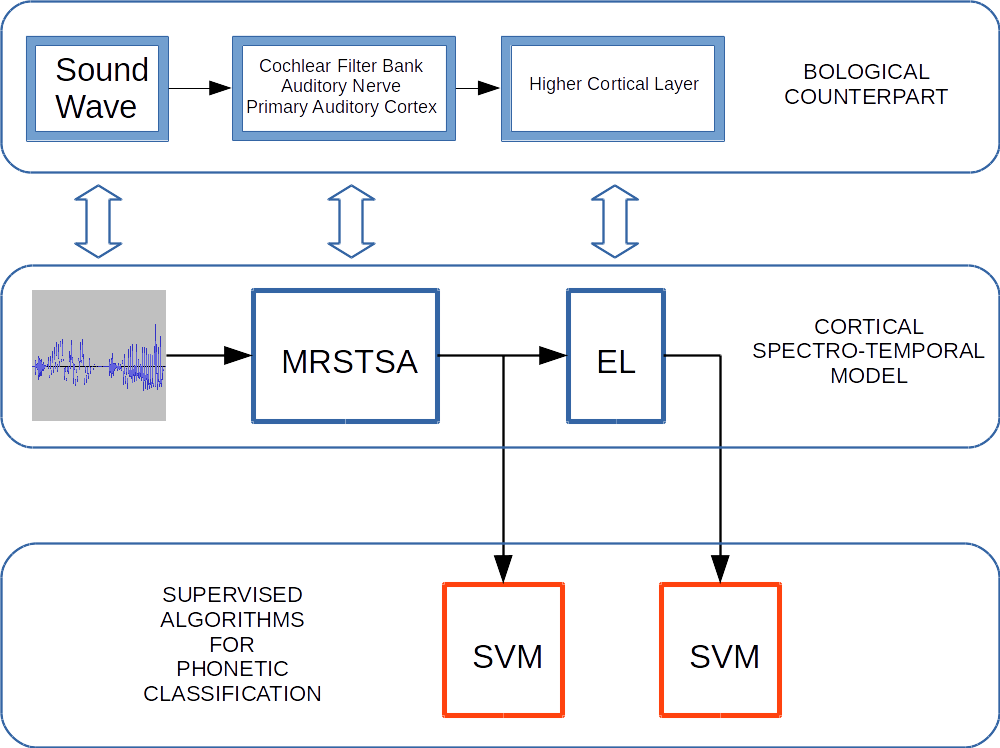
\includegraphics[width=0.7\textwidth]{Experiment.png}
    %\caption{Configuración experimental para probar el desempeño en las tareas de clasificación de palabras.
    %Las ondas de sonido son procesadas por el algoritmo \gls{mrstsa}.
    %Las salidas desde el \gls{mrstsa} son procesadas por el \gls{el}.
    %Las tareas de clasificación de palabras son realizadas sobre ambas salidas por medio del algoritmo \gls{svm}.
    %Cada sección en el \gls{cstm} tiene su contrapartida biológica.}
    %%\caption{Experimental setup to test word classification task performances.
    %%Sound waves are processed by the \gls{mrstsa} algorithm.
    %%The outputs from the \gls{mrstsa} are processed by the \gls{el}.
    %%Word classification tasks are performed on both outputs by the \gls{svm} algorithm.
    %%Each section in the \gls{cstm} has its biological counterpart.}
    %\label{fig:Experiment}
%\end{figure}

%\pagebreak

%En el procedimiento experimental primero entrenamos el \gls{el} con un corpus original de 500 palabras desde un vocabulario de 5 palabras con 10 voces diferentes (8 masculinas y 2 femeninas) generadas por el sintetizador de habla \gls{festival} \cite{festival2014}. Luego, procesamos el mismo corpus con el \gls{el} en modo de inferencia. En tal modo, el \gls{el} procesa la información con las propiedades de aprendizaje deshabilitadas. De esta manera, durante la inferencia, el \gls{el} no modificó sus sinapsis y sólo devolvió patrones de activación en respuesta a los estímulos que recibió. Luego utilizamos las salidas desde el \gls{mrstsa} y desde el \gls{el} en modo de inferencia para entrenar los clasificadores \gls{svm}. El desempeño de los entrenamientos con validación cruzada se muestra en la Tabla \ref{SVM_Training}.

%%In the experimental procedure we first trained the \gls{el} with an original corpus of 500 words from a vocabulary of 5 words with 10 different voices (8 males and 2 females) generated by \gls{festival} Synthesis \cite{festival2014} speech synthesizer. Afterwards, we processed the same corpus with the \gls{el} in inference mode. In such mode, the \gls{el} processed the information with its learning properties disabled. In this manner, during inference, the \gls{el} did not modify its synapses and just returned patterns of activation in response to the stimuli it received. We then used the outputs from the \gls{mrstsa} and the \gls{el} in inference mode to train the \gls{svm} classifiers. The cross validation training performances are shown in Table~\ref{SVM_Training}.

%\begin{table}[h!]
%\centering
%\caption{\gls{svm} 5-fold cross validation training results}
%\begin{tabular}{|l|l|l|}
%\hline
                   %& MRSTSA & Encoder Layer \\ \hline
%Monosyllabic Words & 98.8\% & 99\%          \\ \hline
%Disyllabic Words   & 98\%   & 97.8\%        \\ \hline
%Trisyllabic Words  & 97.6\% & 98\%          \\ \hline
%\end{tabular}
%\label{SVM_Training}
%\end{table}

%\pagebreak

%En una segunda etapa, corrimos el \gls{el} en modelo de inferencia nuevamente, pero esta vez afectamos el corpus original por medio de diferentes tipos de varianzas. Testeamos el desempeño del los clasificadores ya entrenados en presencia de las características devueltas por los algoritmos en repuesta a los corpus afectados por las varianzas introducidas a los corpus originales por medio de Audacity \cite{audacity}. Las varianzas introducidas incluyeron ruido blanco, reverberación y variaciones de tono. 

%%In a second stage, we ran the \gls{el} in inference mode again, but this time we affected the original corpus by means of different kind of variances. We tested the performances of the--already trained--classifiers in the presence of the features returned by the algorithms in response to the corpus affected by the variances which we introduced to original corpora by means of Audacity \cite{audacity}. The variances introduced to the original corpus included white noise, reverberation and pitch variations. 

%Los desempeños de clasificación se muestran en las Figs. \ref{fig:MONO_ACC}, \ref{fig:DI_ACC} and \ref{fig:TRI_ACC}.

%%The classification performances are shown in Figs. \ref{fig:MONO_ACC}, \ref{fig:DI_ACC} and \ref{fig:TRI_ACC}.

%\begin{figure}[h!]
    %\centering
    %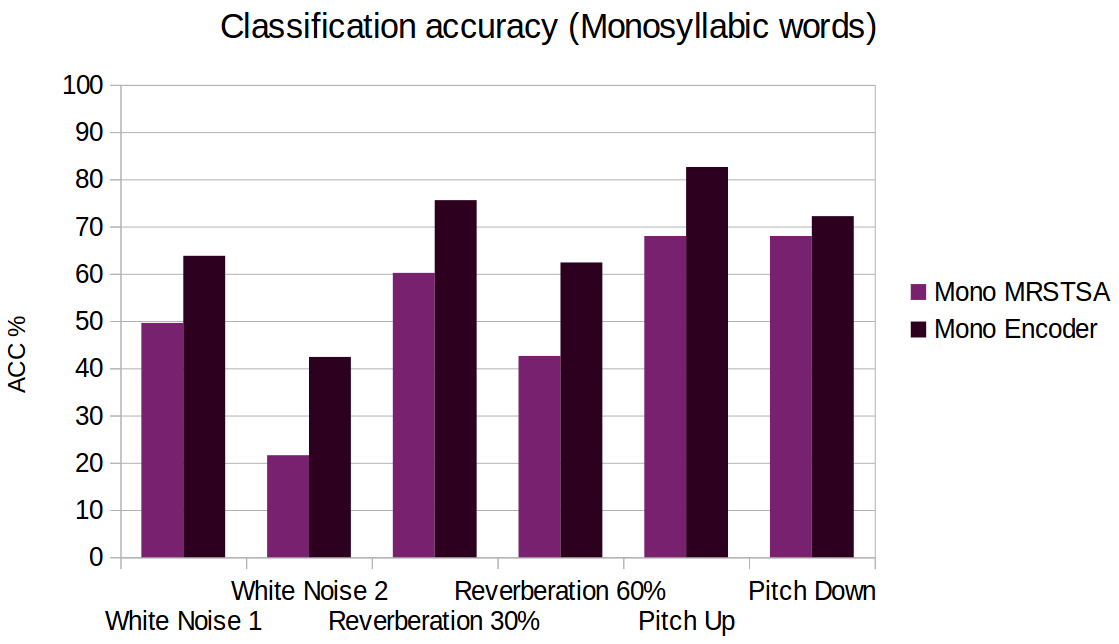
\includegraphics[width=0.9\textwidth]{MONO_ACC.png}
    %\caption{Precisión en la clasificación realizada sobre el \gls{mrstsa} y el \gls{el} contra diferentes varianzas introducidas en las señales originales
    %para \textbf{palabras monosilábicas}.
    %White Noise 1 determina una relación de señal a ruido o \gls{snr} tasa promedio de potencia \gls{rms} de 19.8 dB mientras que White Noise 2 13.8 dB.
    %Reverberation 30\% determina un valor de \gls{rt} de 0.61 segundos mientras que Reverberation 60\% determina un valor de \gls{rt} de 1.78 segundos.
    %Pitch Up determina un cambio de tono desde E a G, mientras que Pitch Down determina un movimiento de tono desde E a C.}
    %%\caption{\gls{mrstsa} and \gls{el} classification accuracies against different variances introduced to the original signals
    %%for \textbf{monosyllabic words}.
    %%White Noise 1 determines a \gls{snr} average \gls{rms} power rate of 19.8 dB while White Noise 2 13.8 dB.
    %%Reverberation 30\% determines a \gls{rt} value of 0.61 seconds while Reverberation 60\% determines a \gls{rt} value of 1.78 seconds.
    %%Pitch Up determines a pitch move from E to G, while Pitch Down determines a pitch move from E to C.}
    %\label{fig:MONO_ACC}
%\end{figure}

%\begin{figure}[h!]
    %\centering
    %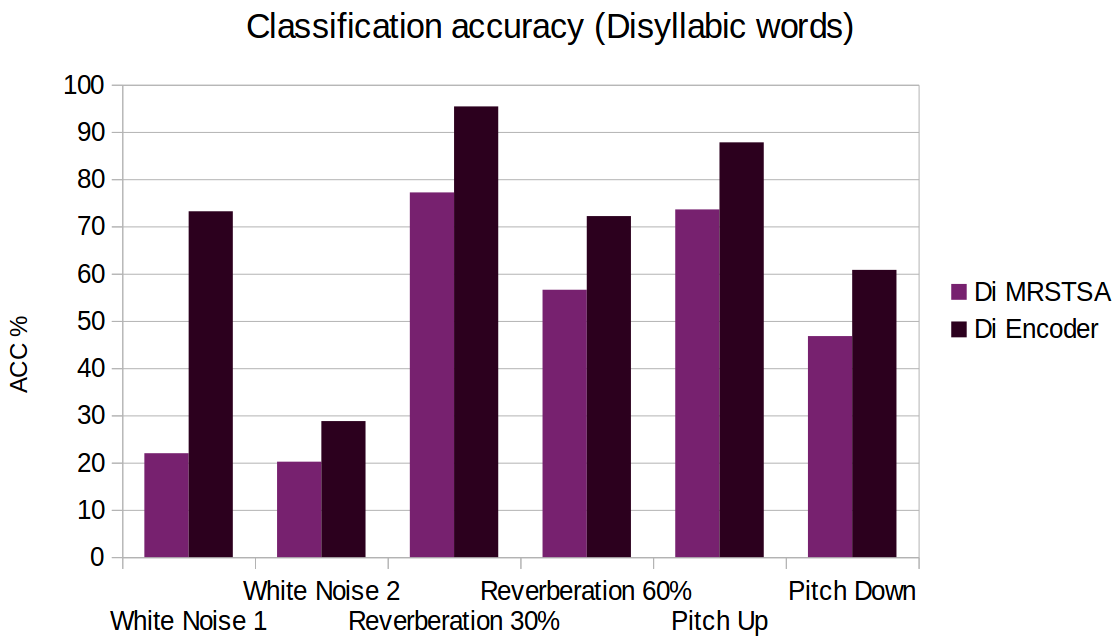
\includegraphics[width=0.9\textwidth]{DI_ACC.png}
    %\caption{Precisión en la clasificación realizada sobre el \gls{mrstsa} y el \gls{el} contra diferentes varianzas introducidas en las señales originales
    %para \textbf{palabras disilábicas}.
    %White Noise 1 determina una relación de señal a ruido o \gls{snr} tasa promedio de potencia \gls{rms} de 19.8 dB mientras que White Noise 2 13.8 dB.
    %Reverberation 30\% determina un valor de \gls{rt} de 0.61 segundos mientras que Reverberation 60\% determina un valor de \gls{rt} de 1.78 segundos.
    %Pitch Up determina un cambio de tono desde E a G, mientras que Pitch Down determina un movimiento de tono desde E a C.}
    %%\caption{\gls{mrstsa} and \gls{el} classification accuracies against different variances introduced to the original signals
    %%for \textbf{disyllabic words}.
    %%White Noise 1 determines a \gls{snr} average \gls{rms} power rate of 19.8 dB while White Noise 2 13.8 dB.
    %%Reverberation 30\% determines a \gls{rt} value of 0.61 seconds while Reverberation 60\% determines a \gls{rt} value of 1.78 seconds.
    %%Pitch Up determines a pitch move from E to G, while Pitch Down determines a pitch move from E to C.}
    %\label{fig:DI_ACC}
%\end{figure}

%\begin{figure}[h!]
    %\centering
    %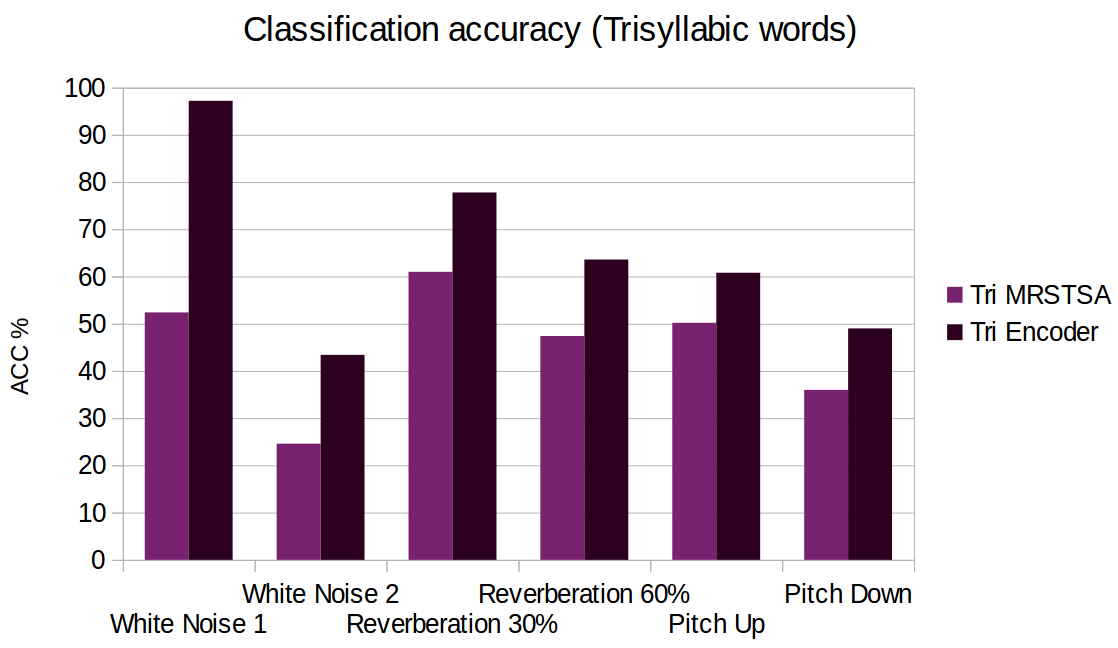
\includegraphics[width=0.9\textwidth]{TRI_ACC.png}
    %\caption{Precisión en la clasificación realizada sobre el \gls{mrstsa} y el \gls{el} contra diferentes varianzas introducidas en las señales originales
    %para \textbf{palabras trisilábicas}.
    %White Noise 1 determina una relación de señal a ruido o \gls{snr} tasa promedio de potencia \gls{rms} de 19.8 dB mientras que White Noise 2 13.8 dB.
    %Reverberation 30\% determina un valor de \gls{rt} de 0.61 segundos mientras que Reverberation 60\% determina un valor de \gls{rt} de 1.78 segundos.
    %Pitch Up determina un cambio de tono desde E a G, mientras que Pitch Down determina un movimiento de tono desde E a C.}
    %%\caption{\gls{mrstsa} and \gls{el} classification accuracies against different variances introduced to the original signals
    %%for \textbf{trisyllabic words}.
    %%White Noise 1 determines a \gls{snr} average \gls{rms} power rate of 19.8 dB while White Noise 2 13.8 dB.
    %%Reverberation 30\% determines a \gls{rt} value of 0.61 seconds while Reverberation 60\% determines a \gls{rt} value of 1.78 seconds.
    %%Pitch Up determines a pitch move from E to G, while Pitch Down determines a pitch move from E to C.}
    %\label{fig:TRI_ACC}
%\end{figure}

%\pagebreak

%En relación con el ruido blanco, introducimos ruido blanco aditivo a la señal original con una tasa de potencia de señal a ruido promedio o \gls{rms} de 19.9 dB (White Noise 1) y 13.8 dB (White Noise 2). En términos de reverberación, modificamos la señal original por medio de valores de \gls{rt} de 0.61 segundos (Reverberation 30\%) y 1.78 segundos (Reverberation 60\%). \gls{rt} es el tiempo que la señal toma para decrecer en su amplitud a 60 dBs por debajo de su valor inicial. En relación a las variaciones de tono, modificamos el tono de la señal en un +20\% (de E a G) (Pitch Up) y en --20\% (de E a C) (Pitch Down).

%%Regarding white noise, we introduced additive white noise to the original signal with a signal-noise average \gls{rms} power rate of 19.9 dB (White Noise 1) and 13.8 dB (White Noise 2). In terms of reverberation, we modified the original signal by means of \gls{rt} values of 0.61 seconds (Reverberation 30\%) and 1.78 seconds (Reverberation 60\%). \gls{rt} Is the time that a signal takes to decrease its amplitude to 60 dBs under its initial value. As regards pitch variations, we modified the signal pitch in +20\% (from E to G) (Pitch Up) and in --20\% (from E to C) (Pitch Down).

%Las Figs. \ref{fig:MONO_ACC}, \ref{fig:DI_ACC} y \ref{fig:TRI_ACC} muestran la exactitud en una tarea de clasificación de 5 vías para palabras mono, di y trisilábicas en los corpus afectadas por ruido blanco, reverberación y variaciones de tono. Como se puede ver en las figuras, el \gls{el} supera al \gls{mrstsa} en todos los casos. Tal comportamiento persiste para palabras multisilábicas.

%%Figs. \ref{fig:MONO_ACC}, \ref{fig:DI_ACC} and \ref{fig:TRI_ACC} show a 5 way word classification accuracy for mono, di and trisyllabic word corpora affected by white noise, reverberation and pitch variations. As can be seen in the figures, the \gls{el} outperforms the \gls{mrstsa} in all cases. Such behavior persists for multisyllabic words.

%La Fig. \ref{fig:AV_ACC} muestra la exactitud promedio en la clasificación a través de todas las varianzas para palabras mono, di y trisilábicas. Como se puede apreciar en la figura, de acuerdo con las barras de \textbf{Error Standard}, el encoder muestra con claridad una superioridad sustenida a través de palabras con diferentes números de sílabas.

%%Fig. \ref{fig:AV_ACC} shows average classification accuracies across all variances for mono, di and trisyllabic words. As can be seen in the figure, according to \textbf{Standard Error} bars, the encoder layer clearly shows a sustained superiority across words with different number of syllables.

%\begin{figure}[h!]
    %\centering
    %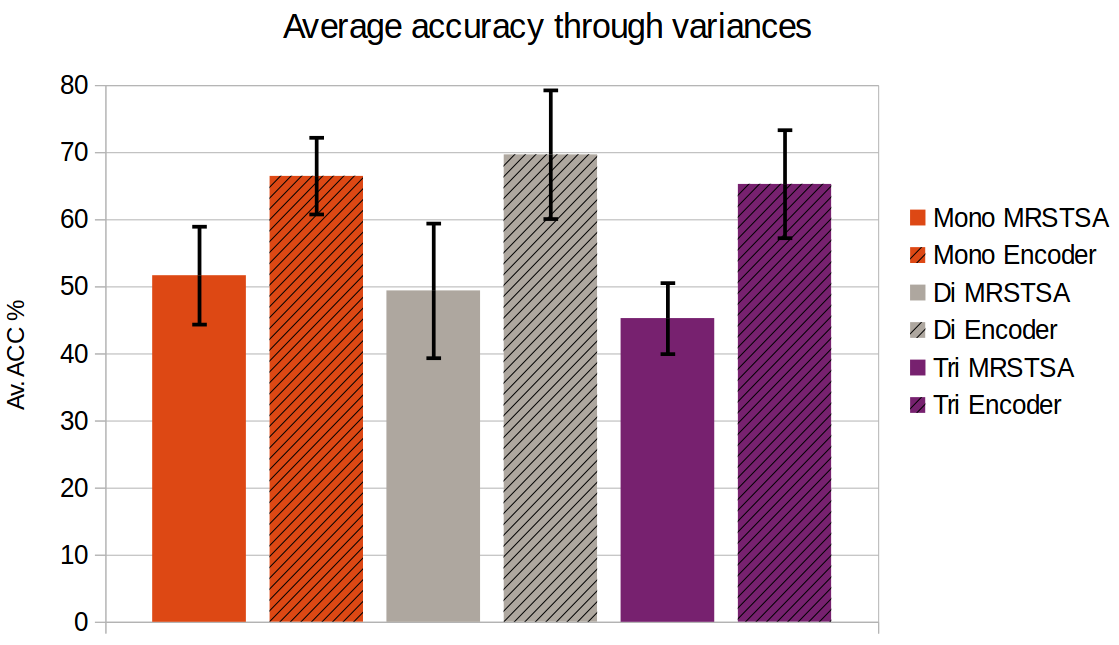
\includegraphics[width=0.9\textwidth]{AV_ACC.png}
    %\caption{Promedio de exactitud en clasificación a través de todas las varianzas para palabras mono, di y trisilábicas con barras de Error Standard.
    %Mono significa palabras monosilábicas, Di significa palabras disilábicas y Tri significa palabras trisilábicas.}
    %%\caption{Average classification accuracies across all variances for mono, di and trisyllabic words with Standard Error bars.
    %%Mono means monosyllabic words, Di means disyllabic words and Tri means trisyllabic words.}
    %\label{fig:AV_ACC}
%\end{figure}

